\section{Analysis Overview}

This measurement uses data corresponding to a BNB exposure of $5.89\times10^{20}$~protons on target (POT), collected during the period 2016--2018 and referred to as ``Runs 1--3'' in many of the subsequent figures. Neutrino-argon interactions are simulated using a custom tune \cite{MicroBooNE:2021ccs} of the \textsc{genie} neutrino event generator v3.0.6 \cite{Andreopoulos:2009rq,GENIE:2021zuu} (based on model set  G18\_10a\_02\_11a) adopted by the MicroBooNE Collaboration. This tune specifically targets CC quasi-elastic (QE) and CC multi-nucleon interaction models and overall has very little direct effect on this NC-focused analysis. \textsc{genie} v3 uses the Berger-Sehgal~\cite{Rein:1980wg,Berger:2007rq} model for resonant production of $\pi^0$ and includes improved agreement with an expanded data set for the $A$-dependence of final state interactions (FSI), updated form factors \cite{Graczyk:2008}, updated diagrams for pion production processes \cite{Berger:2007rq,Kuzmin:2004,Nowak:2009}, and a new tune to neutrino-proton and neutrino-deuterium cross-section data \cite{GENIE:2021zuu}. The MicroBooNE Monte Carlo (MC) prediction further makes use of \textsc{geant4} v4\_10\_3\_03c \cite{GEANT4:2002zbu} for particle propagation and re-interactions within the detector and a custom detector response model all implemented within the LArSoft framework~\cite{Snider_2017}. 

The MicroBooNE data and MC reconstruction chain begins by reading out and processing the ionization charge signals detected on the 8,192 wires that make up the three anode planes of the MicroBooNE LArTPC. The procedure includes noise removal \cite{MicroBooNE:2017qiu} and signal processing as described in \cite{MicroBooNE:2018swd} and \cite{MicroBooNE:2018vro}. Localized regions of interest referred to as ``hits'' are then identified and fit to Gaussian pulses. The collection of these hits and their characteristics such as readout time, wire channel number, and integrated charge are then used as input to the Pandora pattern recognition framework for further processing \cite{Marshall:2015rfa}. The Pandora framework clusters and matches hits across three 2D projected views of the MicroBooNE active TPC volume to form 3D reconstructed objects. These objects are then classified as track-like or shower-like based on a multivariate classifier score and aggregated into candidate neutrino interactions. Pandora also reconstructs a candidate neutrino interaction vertex based on the position and orientation of the reconstructed tracks and showers which represents the most likely position of the neutrino interaction.

Being a surface detector, MicroBooNE is subject to a constant stream of high-energy cosmic rays impinging on the detector that substantially outnumber the neutrino interactions and form the largest background to candidate neutrino interactions. To incorporate the effect of cosmic-ray contamination in the simulation, cosmic ray data recorded \textit{in situ} at MicroBooNE, when the beam is not present, are used as overlays (at the wire signal waveform level) to  simulated neutrino interactions. During the 2.3 ms that it takes to ``drift'' ionization charge associated with neutrino interaction final states across the maximum 2.56 m drift distance, $\mathcal{O}(10)$ cosmic rays are expected to enter the detector. In order to reduce this cosmic-ray contamination, scintillation light recorded by the MicroBooNE photo-detector system is matched to candidate neutrino interactions during reconstruction and is also required to occur in time with the 1.6~$\mu$s long BNB neutrino spill.  

To select a high-purity sample of BNB neutrino NC $1\pi^0$ interactions, a series of topological, pre-selection, and boosted decision tree (BDT)-based selections are applied. This results in two mutually exclusive final selection topologies: $2\gamma1p$, which targets two photons and one proton in the final state, and $2\gamma0p$, which targets two photons and zero protons in the final state. The different selection stages are described below, along with the details of the systematic uncertainty evaluation. 

\subsection{Topological Selection and Pre-Selection}

The event selection begins with topology-based criteria for candidate neutrino interactions identified by Pandora and targets two mutually exclusive topological definitions: (a) two showers and one track ($2\gamma 1p$), and (b) two showers and zero tracks ($2\gamma 0p$). The two showers correspond to the photons expected from $\pi^0$ decay. The presence of a track corresponds to a reconstructed proton exiting the nucleus while the zero-track case suggests either a low-energy proton that is not reconstructed or no charged hadrons at all exiting the nucleus. 

Once events with the desired signal topologies are identified, a series of loose ``pre-selection'' requirements is applied to reduce obvious backgrounds or mis-reconstructed events. These pre-selection requirements include shower energy thresholds of 30~MeV for the leading shower and 20~MeV for the subleading shower in both topologies. The pre-selection also requires that the reconstructed neutrino interaction point be contained in a fiducial volume, defined as at least 5~cm away from any TPC wall, in order to help reduce the number of selected events with tracks that exit the detector. For the 2$\gamma$1p topology, the non-zero conversion distance of photons is explicitly used by requiring that each shower has a reconstructed start point of at least 1~cm from the reconstructed neutrino interaction vertex. Typically the reconstructed neutrino interaction vertex is identified as the start of the reconstructed proton candidate track. In order to remove a very small number of poorly reconstructed events in which the candidate track is not consistent with the hypothesis of originating from the candidate neutrino interaction vertex, a requirement is placed to ensure the track start point is always within 10~cm of the reconstructed neutrino interaction vertex. The efficiency of selecting NC $1\pi^0$ + 0 (1)p events using these pre-selection requirements is 21.5\% (19.9\%). Note that the efficiency of the 1p selection is lower because of the additional requirements placed on the track reconstruction. 

\subsection{Boosted Decision Tree-Based Selection}
After applying the pre-selection requirements, the remaining signal and background are further differentiated and separated using two tailored BDTs trained on simulation. The gradient boosting algorithm XGBoost \cite{Chen:2016:XST:2939672.2939785} is used to train each of the BDTs. They take as input various reconstructed kinematic, geometric, and calorimetric variables both for the signal (defined as an NC interaction with identically one $\pi^0$ in the final state) and for the background interactions. Because the two tailored BDTs target different topologies, notably including one track in the case of $2\gamma1p$ and zero tracks in the case of $2\gamma0p$, the signal definitions used for the two BDTs are slightly different. NC $\pi^0$ events with exactly one proton with true kinetic energy above 20~MeV are used as the training signal for the $2\gamma1p$ BDT while NC $\pi^0$ events with no protons with true kinetic energy above 20 MeV are used as the training signal for the $2\gamma0p$ BDT. We note that the 20 MeV threshold used in the BDT training is lower than the 50 MeV proton kinetic energy threshold used later during cross-section extraction, as during training we are aiming to push the threshold as low as possible. Each BDT is trained on ten reconstructed variables. Due to the existence of a proton candidate track in the $2\gamma1p$ sample, these ten variables differ for each BDT. They are listed below.\\

\noindent \textbf{Variables used in both $\bm{2\gamma1p}$ and $ \bm{2\gamma0p}$ BDTs:}
\begin{itemize}
    \item Leading and subleading shower impact parameters: The perpendicular distance between the back-projection of the reconstructed shower and the candidate neutrino interaction point which is a metric of how well each shower ``points'' back to the reconstructed neutrino interaction point. 
    \item Leading and subleading shower conversion distances: Defined as the distance between the reconstructed start of the shower and reconstructed neutrino interaction point. 
    \item Reconstructed energy of the leading shower.
\end{itemize}
\noindent \textbf{Variables used in only the $\bm{2\gamma1p}$ BDT:}
\begin{itemize}
    \item Reconstructed track length.
    \item Reconstructed track vertical angle: Defined as the arctangent of the track direction in the vertical plane with respect to the beam axis.
    \item Distance from track end to TPC wall: Calculated as the shortest distance to the closest TPC wall.
    \item Reconstructed mean energy deposition per unit length ($dE/dx$) of the track.
    \item Ratio of $dE/dx$ of the first half of track to that of the second half of the track: A metric for identifying stopping proton tracks that contain a Bragg peak.
\end{itemize}
\noindent \textbf{Variables used in only the $\bm{2\gamma0p}$ BDT:}
\begin{itemize}
    \item Reconstructed energy of the subleading shower.
    \item Leading and subleading shower geometric length per unit energy: The ratio of each shower's geometric length to its reconstructed energy. The geometric length is an estimate of the 3D extent of the electromagnetic shower. 
    \item Pandora ``neutrino score'': A multivariate classifier in the Pandora reconstruction suite which scores all reconstructed neutrino candidates based on their geometric and kinematic features as to how likely a candidate is due to a neutrino interaction or cosmic in origin.
    \item Reconstructed leading shower vertical angle: Direction in the vertical plane with respect to the beam axis.
\end{itemize}

By construction, BDT scores lie on the interval of [0, 1]. After training, the resulting BDT score distributions, tested on a statistically independent simulation and data set, are shown in Fig.~\ref{fig:bdt_responses}. The simulation and data points agree across the full range of BDT classifier score within systematic and statistical uncertainties (the definition of these systematic uncertainties is described in detail in Sec.~\ref{sec:systematics}). The bimodal distribution of the $2\gamma1p$ BDT response indicates greater separation power between signal and background compared to that for $2\gamma0p$ because the addition of the reconstructed track gives access to an entirely separate handle on background rejection. For this and subsequent MC simulation comparisons to data, the simulation predictions are broken down into the following eight categories, based on \textsc{genie} truth-level information:
\begin{itemize}
    \item NC 1$\pi^0$: All neutral current interactions that produce one exiting $\pi^0$ regardless of incoming neutrino flavor. This is our targeted signal selection, and it is further split into two sub-categories, ``NC 1$\pi^0$ Coherent'' and ``NC 1$\pi^0$ Non-Coherent'' contributions, based on their interaction types. Non-Coherent scattering occurs when a neutrino interacts with a nucleon inside the argon nucleus, potentially knocking out one or more nucleons. In coherent scattering the neutrino interacts with the nucleus as a whole, leaving it in its ground state. This interactions occurs with low momentum-transfer, and as such the resulting $\pi^0$ tends to be very forward relative to the incoming neutrino beam.
    \item NC $\Delta \rightarrow N\gamma$: Leading Standard Model source of NC single-photon production below 1~GeV originating from radiative decay of the $\Delta(1232)$ baryon.
    \item CC $\nu_\mu 1 \pi^0$: All $\nu_\mu$ CC interactions that have one true exiting $\pi^0$.
    \item CC $\nu_e/\overline{\nu}_{e}$ Intrinsic: All CC $\nu_e$ or $\overline{\nu}_{e}$ interactions regardless of whether or not a $\pi^0$ was emitted. 
    \item BNB Other: All remaining BNB neutrino interactions that take place in the active TPC volume of MicroBooNE and are not covered by the above five categories, such as multiple $\pi^0$ events and $\eta$ meson decay. See section \ref{sec:backgrounds} for more details.
    \item Dirt (Outside TPC): All BNB neutrino interactions that take place outside the MicroBooNE active TPC but have final states that enter and interact inside the active TPC detector. This can originate from scattering off liquid argon in the cryostat vessel outside the active TPC volume or from interactions in the concrete and ``dirt'' surrounding the cryostat itself. 
    \item Cosmic Data: Coincident cosmic ray interactions that take place during a BNB spill but without any true neutrino interaction present.
\end{itemize}

The final NC $1\pi^0$-enriched samples are selected by placing a requirement on the BDT score distribution that maximizes the product of NC $1\pi^0$ signal efficiency and purity. This corresponds to a threshold on the BDT scores of $>0.854$ and $>0.950$ for $2\gamma1p$ and $2\gamma0p$, respectively.  The final distributions are provided and discussed in Sec.~\ref{finaldistr}.

\begin{figure}[h]
    \centering 
    \begin{subfigure}{0.49\textwidth}
        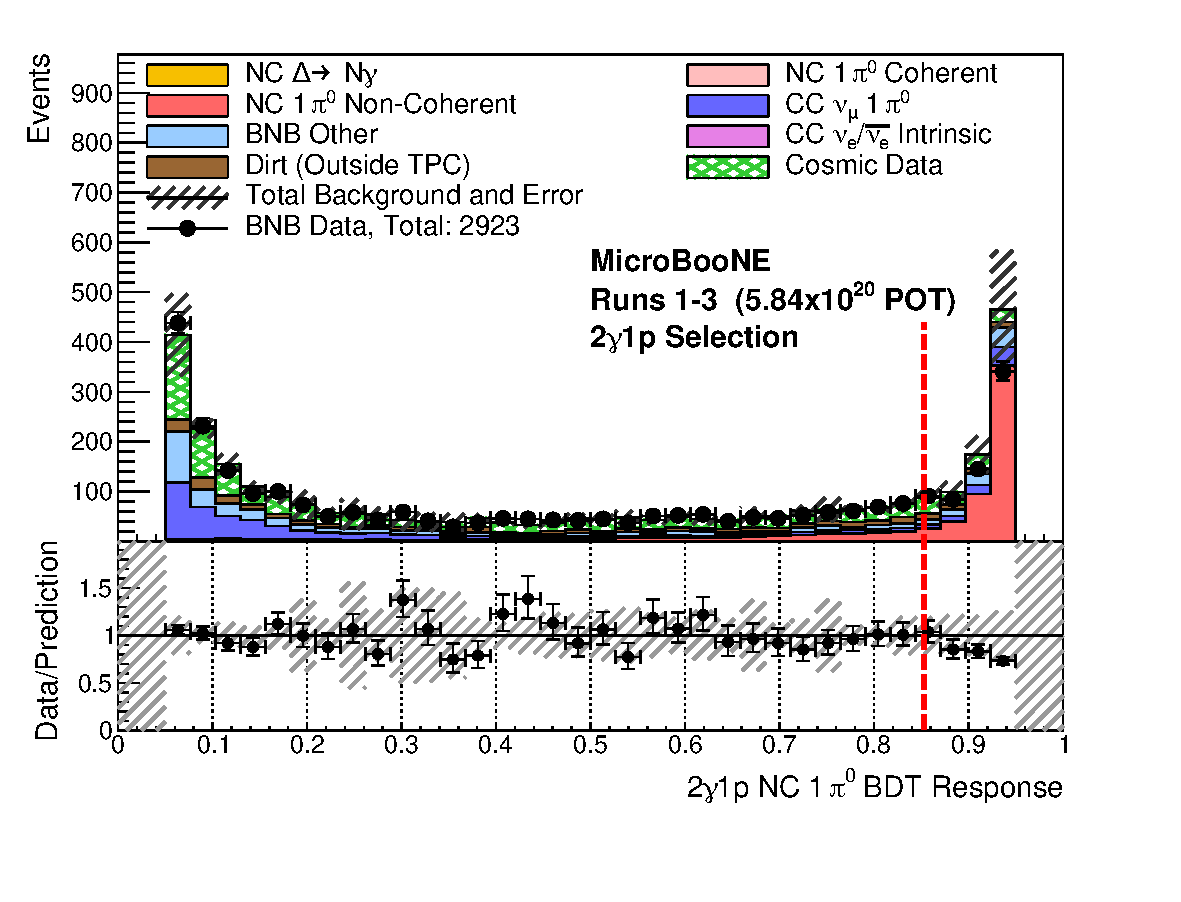
\includegraphics[width = \textwidth]{fig1a_pigLEE_combined_datamc_Data2g1pFiltered_2gamma1pNC1pi0BDTResponse_stage_1WineCheese_v1.pdf}
        \vspace{-1cm}
        \caption{$2\gamma 1p$}
        %\label{fig:bdt_2g1p}
  \end{subfigure} 
  \begin{subfigure}{0.49\textwidth}
      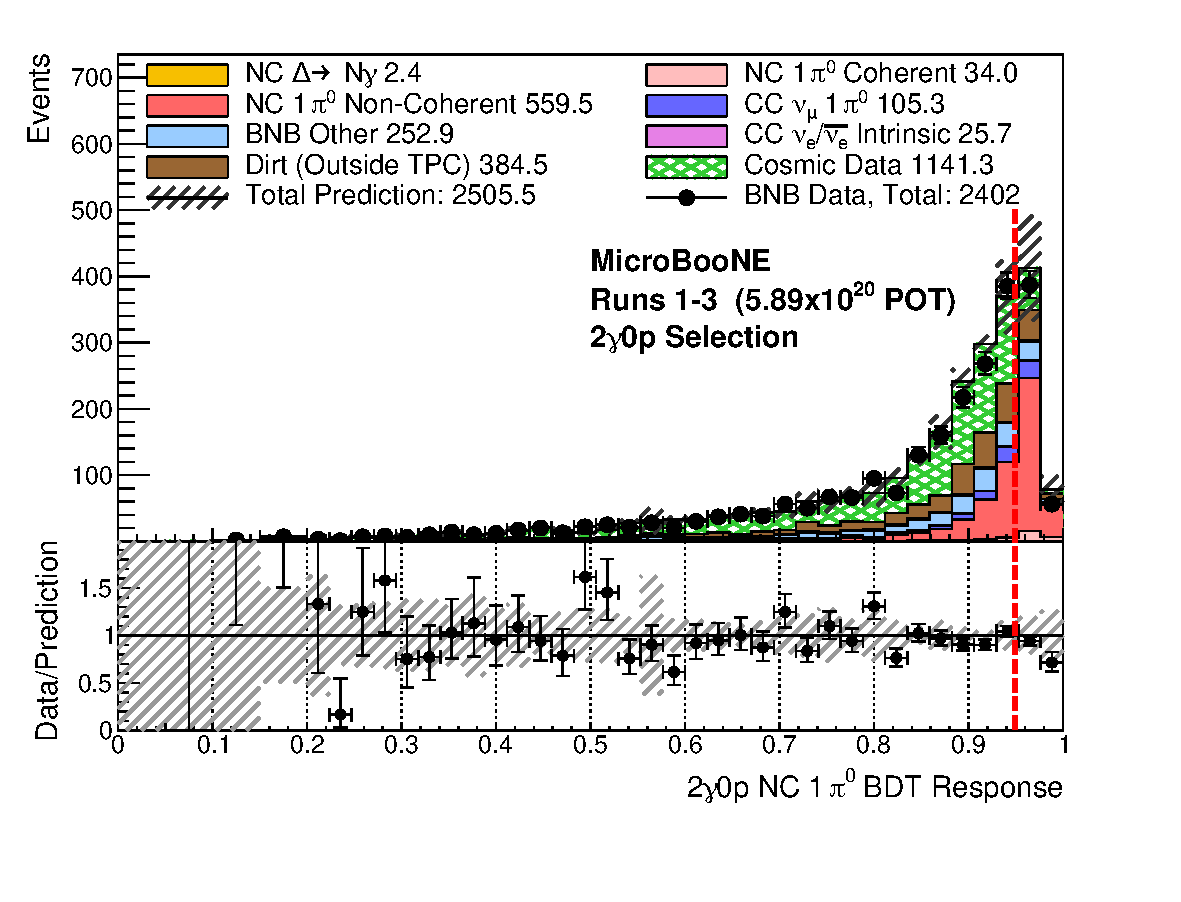
\includegraphics[width = \textwidth]{fig1b_pigLEE_2g0p_combined_datamc_Data2g0pFiltered_2gamma0pNC1pi0BDTResponse_stage_1WineCheese_v1.pdf}
      \vspace{-1cm}
        \caption{$2\gamma 0p$}
        %\label{fig:bdt_2g0p}
  \end{subfigure}
  \caption{The BDT classifier score for (a) $2\gamma 1p$ and (b) $2\gamma 0p$ targeted selections. Higher scores indicate more NC $1\pi^0$ signal-like events, and lower scores indicate more background-like events. The red vertical lines indicate the threshold positions, keeping all events to the right, for the final selections.}
  \label{fig:bdt_responses}
\end{figure}

\subsection{Systematic Uncertainty Evaluation}
\label{sec:systematics}
Systematic uncertainties on the MC simulation prediction include contributions from uncertainties in the neutrino flux, the cross-section modeling, hadron re-interactions, detector effects, and the effect of finite statistics used in the background predictions (both simulations and cosmic ray data).

The flux systematic uncertainties incorporate hadron production uncertainties where the Booster proton beam hits the beryllium target, uncertainties on pion and nucleon scattering in the target and surrounding aluminum magnetic focusing horn of the BNB, and mismodeling of the horn current. Following \cite{MicroBooNE:2019nio}, 
these are implemented by reweighting the flux prediction according to neutrino type, parentage, and energy, and studying the propagated effects on the final event distributions. 

The cross-section uncertainties incorporate modeling uncertainties on the \textsc{genie} prediction~\cite{MicroBooNE:2021ccs,Andreopoulos:2009rq,GENIE:2021zuu}, evaluated by \textsc{genie} reweighting tools. The default \textsc{genie} uncertainties on NC resonant production arising from NC resonant vector and axial mass parameters of $m_V = 0.840 \pm 0.084 $ GeV and $m_A = 1.120 \pm 0.224 $ GeV, respectively, were assumed.  \textsc{genie} uses an effective cascade empirical model for hadronic final-state interactions, called \emph{hA2018}, which allows for reweighting to estimate the effect on final distributions. For more information on cross-section uncertainties in MicroBooNE, please see \cite{MicroBooNE:2021ccs}.

The hadron-argon reinteraction uncertainties are associated with the propagation of hadrons through the detector, as modeled in \textsc{geant4} \cite{GEANT4:2002zbu}. Both charged pions and proton reinteractions during propagation were considered and their impact estimated using the \textsc{geant4reweight} tool \cite{Calcutt:2021zck}.

The detector modeling and response uncertainties are evaluated using MicroBooNE's novel data-driven technique for assessing and propagating LArTPC detector-related systematic uncertainties \cite{MicroBooNE:2021roa}. This approach uses \textit{in situ} measurements of distortions in the TPC wire readout waveform signals -- caused by detector effects such as electron diffusion, electron drift lifetime, electric field, and the electronics response -- to parameterize these effects at the TPC wire level. This provides a detector model-agnostic way to study and evaluate their effects on the high level variables and, subsequently, the final event distributions. Additional detector systematics corresponding to variations in the charge recombination model, the scintillation light yield, and space charge effects~\cite{MicroBooNE:2019koz,MicroBooNE:2020kca} are separately evaluated and also included.

\subsection{Shower Energy Calibration} 

Electromagnetic shower reconstruction in LArTPCs is known to be a lossy process primarily due to mis-clustering and thresholding effects. Current reconstruction algorithms often miss small, low-energy hits in an electromagnetic shower when clustering objects, and some of the hits that are reconstructed may fall below the energy threshold. On average, these effects are expected to yield shower energy losses of approximately 20\% \cite{caratelli2018}. This can be seen in Fig.~\ref{fig:shower_energy_correction}, which shows true and reconstructed shower energy for a dedicated high statistics sample of simulated true NC 1$\pi^0$ events, where the reconstructed shower energy falls systematically below the true shower energy in simulation. By performing a linear fit to the most probable values of reconstructed shower energy in bins of true shower energy, shown as the pink straight line in Fig.~\ref{fig:shower_energy_correction}, a correction factor is extracted which brings the reconstructed values closer to expectation. This fit results in an energy correction that is applied to all reconstructed showers,
\begin{equation}\label{eqn:ncpi0_energy_corr_factor}
    E_{\textrm{corr}} = (1.21 \pm 0.03)E_{\textrm{reco}} + (9.88 \pm 4.86) \ \textrm{MeV},
\end{equation}
and represents a correction of approximately 20\%, as expected.

\begin{figure}
%    \centering
    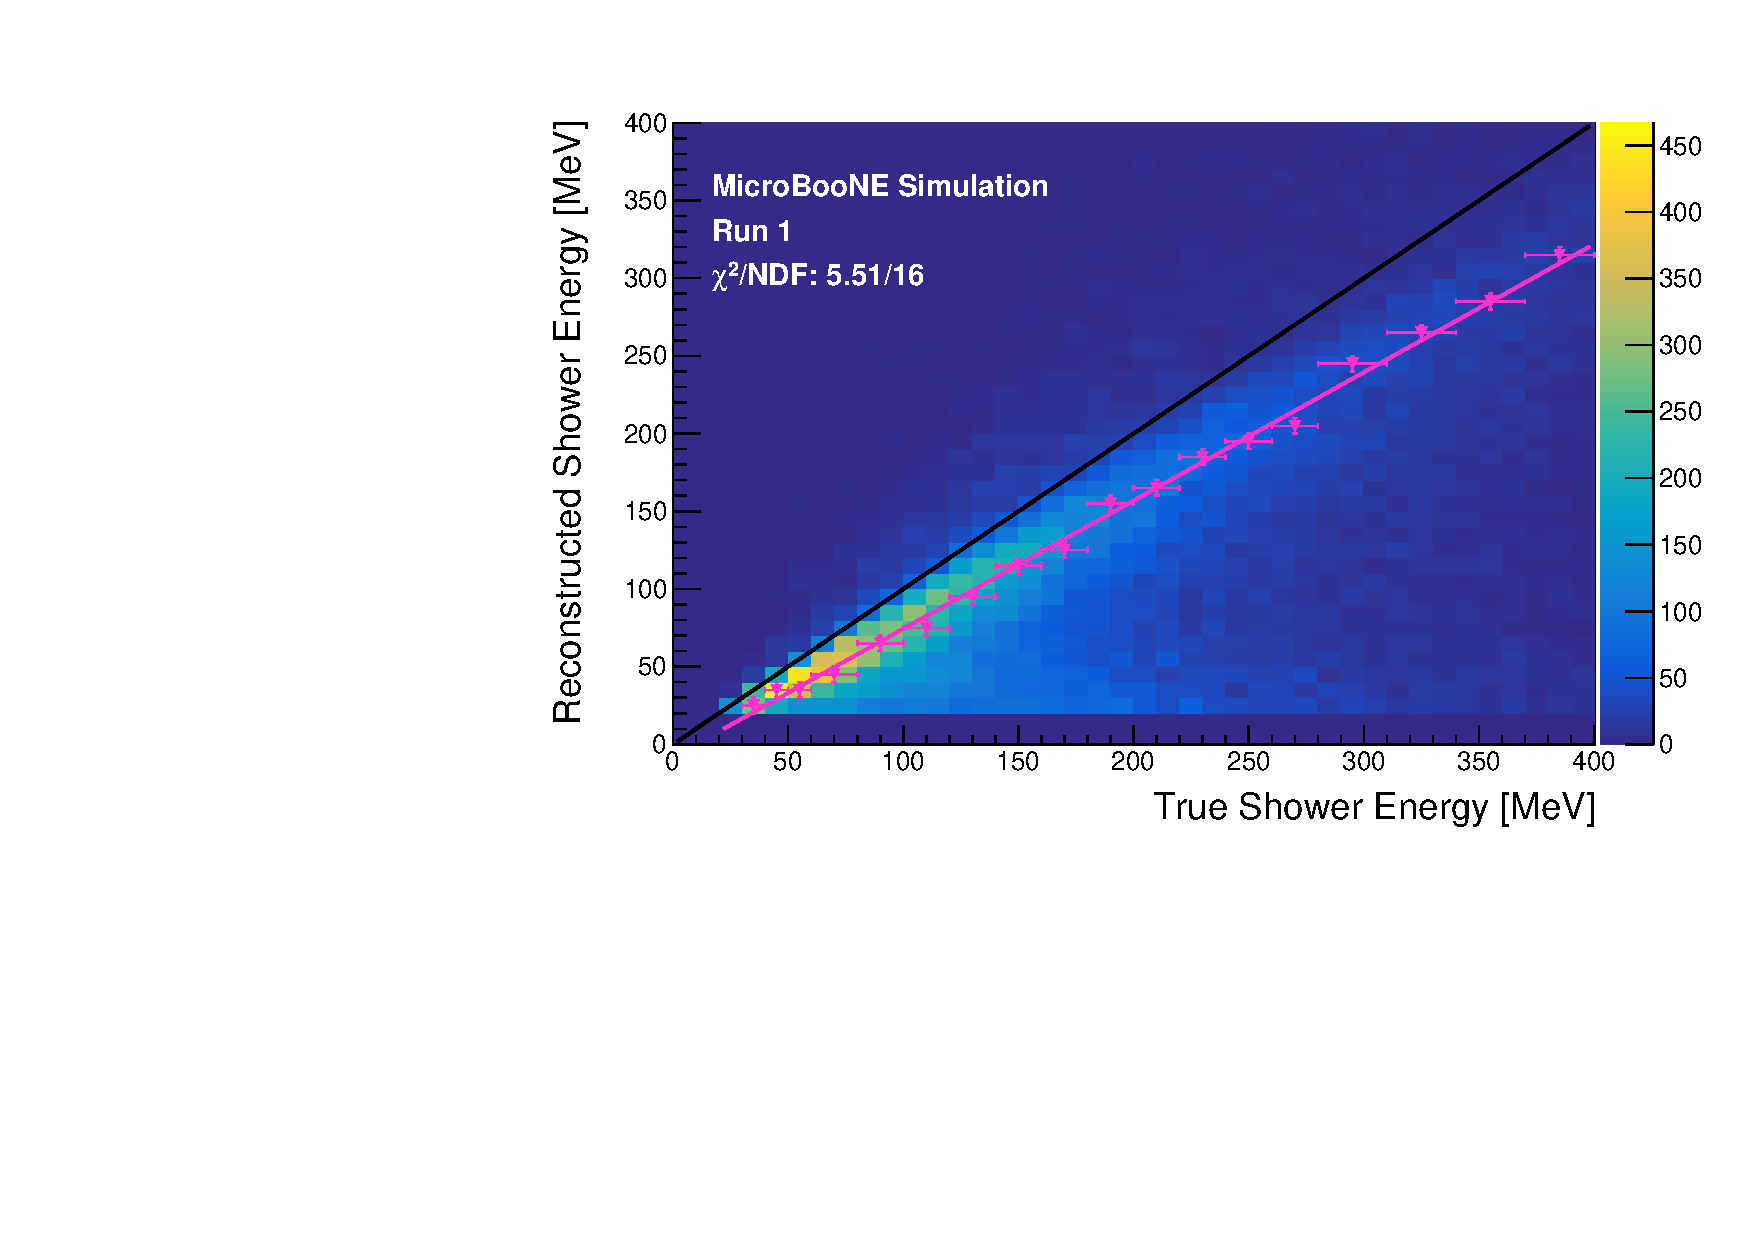
\includegraphics[width=0.48\textwidth]{fig2_plot_max_run1.pdf}
    \caption{Reconstructed shower energy vs. true shower energy for a dedicated high statistics sample of simulated true NC $1\pi^0$ events. Only showers with a reconstructed energy of at least $20$~MeV are considered.}
    \label{fig:shower_energy_correction}
\end{figure}

\subsection{Final Selected Spectra}
\label{finaldistr}

\begin{figure}[h!]
    \centering 
    \begin{subfigure}{0.49\textwidth}
        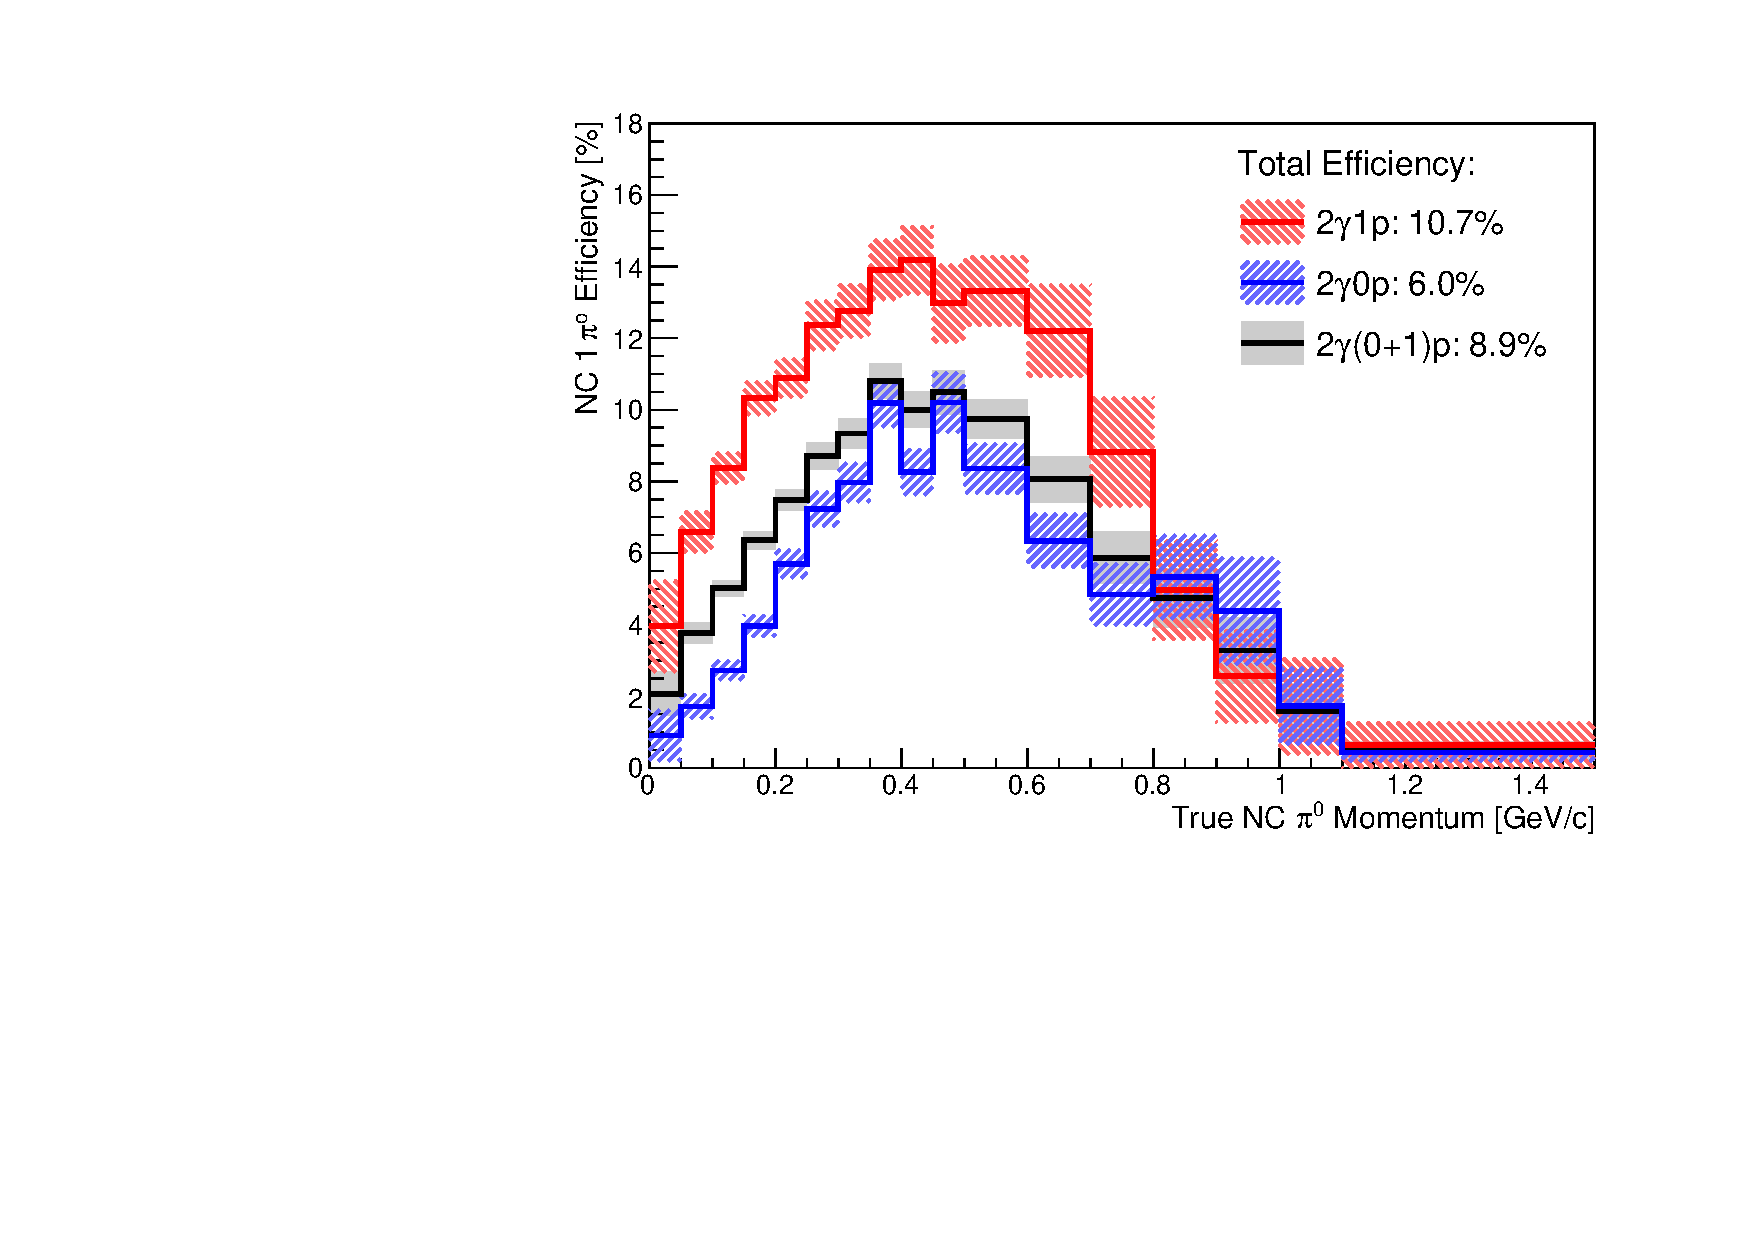
\includegraphics[width = \textwidth]{fig3a_updated_ncpi0BDT.pdf}
        \label{fig:ncpi0_eff_mom}
        \caption{$\pi^0$ momentum dependence}
  \end{subfigure} 
  
  \begin{subfigure}{0.49\textwidth}
        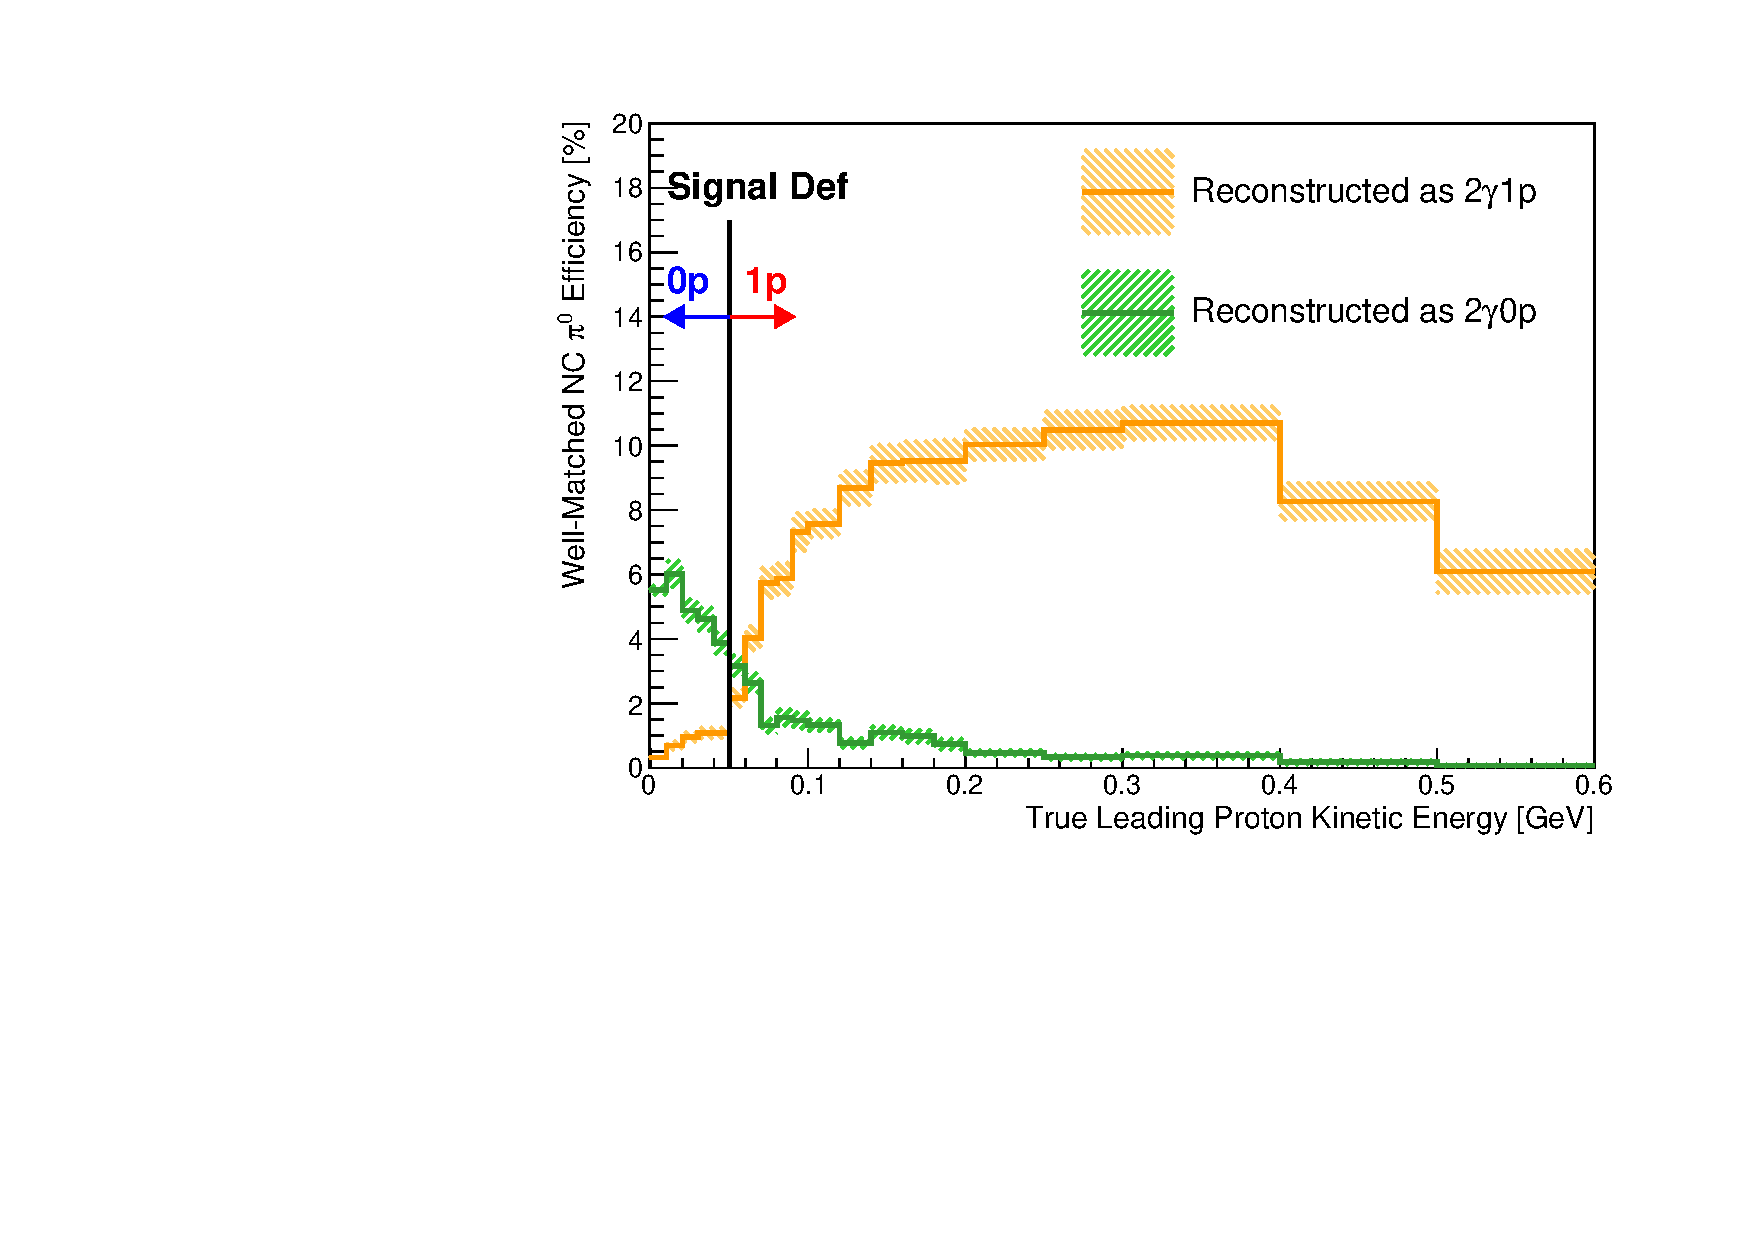
\includegraphics[width = \textwidth]{fig3b_updated_NCPi0ProtonBDT2.pdf}
        \label{fig:ncpi0_eff_pro}
        \caption{Proton kinetic energy dependence}
  \end{subfigure}
  \caption{(a) Efficiencies of the final $2\gamma1p$, $2\gamma0p$ and combined $2\gamma(0+1)p$ selections as a function of true $\pi^0$ momentum. (b) Efficiencies as a function true leading exiting proton kinetic energy for all NC1$\pi^0$ events that are reconstructed as either $1p$ or $0p$. Events in which there are no exiting protons are included in the first bin. As can be seen, a threshold of $\approx$ 50 MeV proton kinetic energy is where events start to shift between the $2\gamma0p$ and $2\gamma1p$ selections which was subsequently chosen as the signal definition for $0p$ and $1p$ signal events.}
  \label{fig:ncpi0_eff}
\end{figure}

After applying the BDT requirements, 1130 selected data events remain with 634 and 496 falling into the $2\gamma1p$ and $2\gamma0p$ selections, respectively. For the $2\gamma 1p$ selection, the BDT score requirement efficiency is 85.6\% and the purity is 63.5\% while for the $2\gamma 0p$ selection, the efficiency and purity are 58.8\% and 52.9\%, respectively. The $2\gamma 1p$ and $2\gamma 0p$ BDT selection efficiencies and purities are both calculated relative to their signal definition, with proton multiplicity counted with a kinetic energy threshold of 50 MeV. The efficiencies at each stage of the analysis are provided in Table~\ref{tab:efficiencies}, and the total efficiency for each selection is shown as a function of (a) true $\pi^0$ momentum and (b) true proton kinetic energy in Fig.~\ref{fig:ncpi0_eff}. Overall, the $1p$ selection is more efficient and of higher signal purity relative to the $0p$ selection due to the existence of a reconstructed particle track which greatly helps to tag the neutrino interaction point and reject backgrounds. This track information, particularly track calorimetry, provides an additional handle on the neutrino interaction mode; a proton-like track is highly indicative of an NC $1\pi^0$ interaction whereas CC interactions generally have a muon track in the final state. 


\begin{figure}[h]
    \centering 
    \begin{subfigure}{0.49\textwidth}
        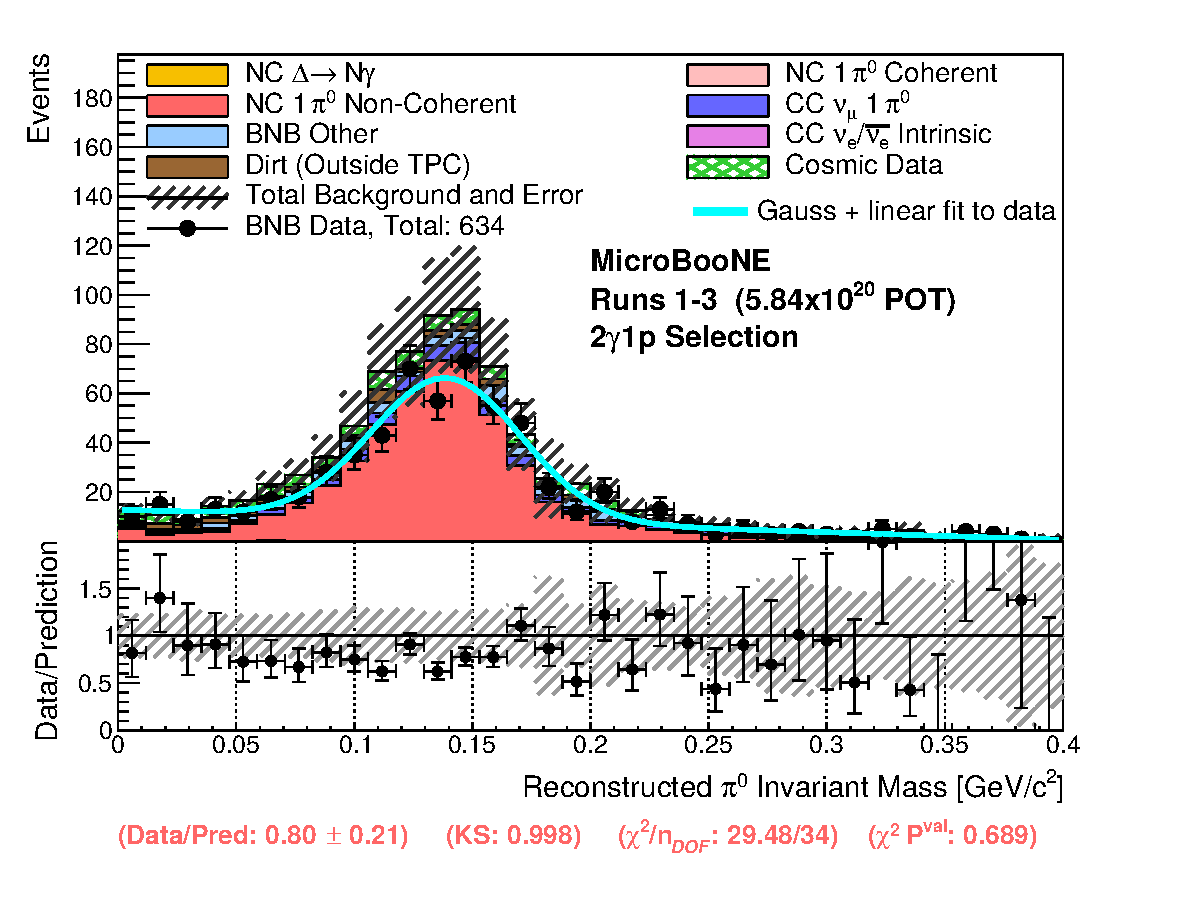
\includegraphics[trim={0 1.5cm 0 0},clip,width = \textwidth]{fig4a_pigLEE_combined_datamc_Data2g1pFiltered_Reconstructedpi0InvariantMassGeVc2_stage_2WineCheese_v1_WFIT_EDIT.pdf}
        \caption{$2\gamma 1p$}
        \label{fig:ncpi0_invar_2g1p}
  \end{subfigure} 
  \begin{subfigure}{0.49\textwidth}
        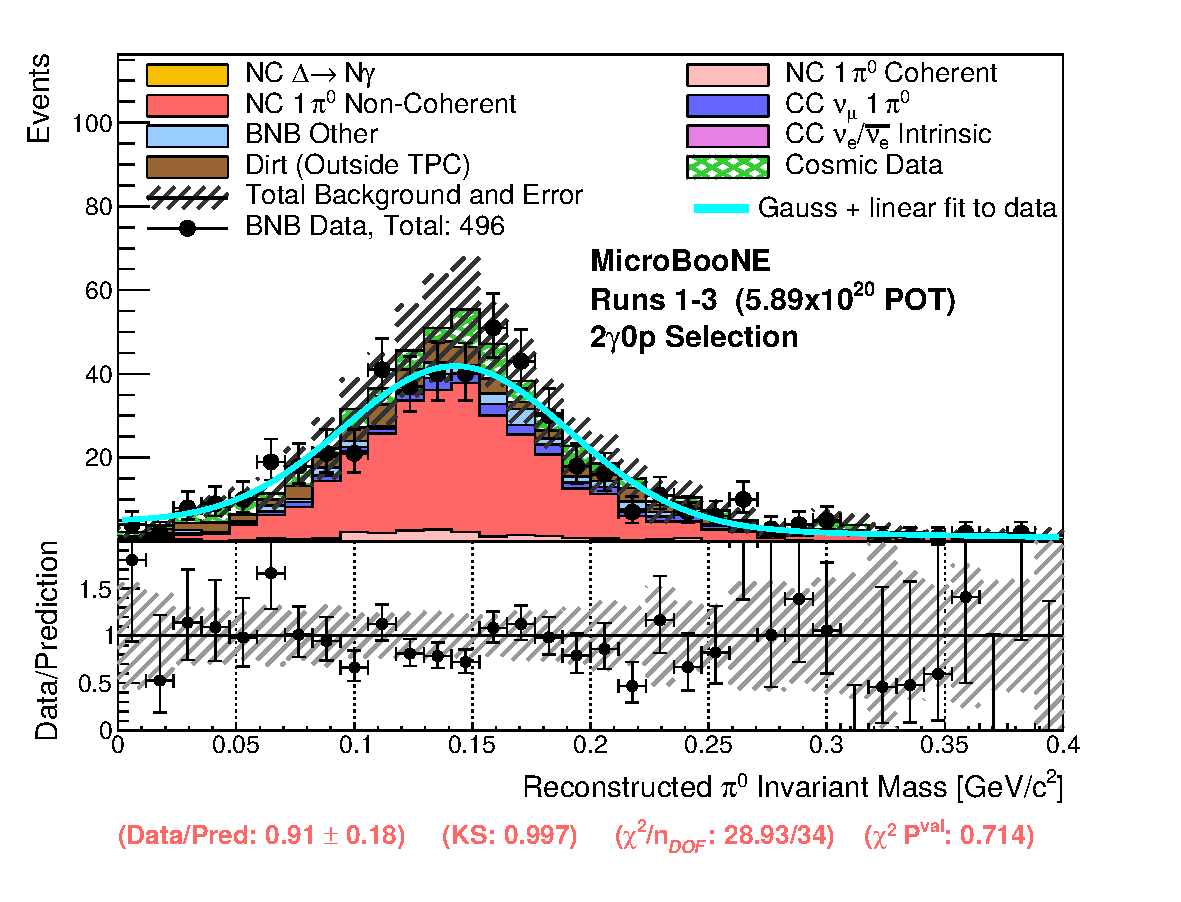
\includegraphics[trim={0 1.5cm 0 0},clip, width = \textwidth]{fig4b_pigLEE_2g0p_combined_datamc_Data2g0pFiltered_Reconstructedpi0InvariantMassGeVc2_stage_2WineCheese_v1_WFIT_EDIT.pdf}
        \caption{$2\gamma 0p$}
        \label{fig:ncpi0_invar_2g0p}
  \end{subfigure}
  \caption{The reconstructed diphoton invariant mass for both the (a) $2\gamma1p$ and (b) $2\gamma0p$ final selected data. The result of fitting a Gaussian plus linear function to the data is shown in cyan.}
  \label{fig:ncpi0_invar}
\end{figure}

\begin{table}[h!]
     \caption{NC $1\pi^0$ efficiencies for the $2\gamma1p$ and $2\gamma0p$ selections. The topological and combined efficiencies are evaluated relative to the defined exclusive $2\gamma1p$ and $2\gamma0p$ signal definitions, inside the active TPC. The pre-selection and BDT selection efficiencies are evaluated relative to their respective preceding selection stage. The final efficiencies are the combined total efficiency for each selection.}
%    \centering
    \begin{tabular}{lrrr}
    \hline\hline
        Selection Stage &  $2\gamma1p$ eff. & $2\gamma0p$ eff. \\ \hline
        Topological & 62.5\% & 47.4\%  \\
        Pre-selection & 19.9\% & 21.5\% \\
        BDT Selection & 85.6\% & 58.8\%  \\ \hline
        Final Efficiencies & 10.7\% & 6.0\%  \\ \hline\hline
    \end{tabular}
    \label{tab:efficiencies}
\end{table}

The resulting distributions as a function of the reconstructed two-photon invariant mass are shown in Fig.~\ref{fig:ncpi0_invar}. The invariant mass is reconstructed from the energy and direction of the two photon candidate showers as
\begin{equation}
   M_{\gamma \gamma}^2 = 2 E_{\gamma 1} E_{\gamma 2} (1- \cos \theta_{\gamma\gamma}),  
   \label{eq:invariant_mass}
\end{equation}
where $\cos \theta_{\gamma\gamma}$ is the opening angle between the two showers. For the $2\gamma1p$ case where a track has been identified as a candidate proton, the directions of the showers and thus the opening angle between them are calculated by constructing the direction between the candidate neutrino interaction point and the shower start point. For the $2\gamma0p$ selection, however, no such candidate track exists. Instead, the shower direction and opening angle are entirely estimated from the geometric shape of the showers themselves. 

A Gaussian-plus-linear fit is performed to each observed distribution in data to extract the reconstructed $\pi^0$ invariant mass while taking into account the non-$\pi^0$ background contamination. For the $2\gamma 1p$ event sample, this fit gives a Gaussian mean of 138.9$\pm$2.1~MeV/$c^2$ with a width of 31.7$\pm$2.4~MeV/$c^2$. For the $2\gamma 0p$ event sample, the corresponding fit gives a Gaussian mean of 143.3$\pm$3.2~MeV/$c^2$ with a width of 47.9$\pm$4.9~MeV/$c^2$. As a goodness-of-fit test, the resulting $\chi^2$ per degree of freedom is 1.20 and 1.45 for the $2\gamma 1p$ and $2\gamma 0p$ fits, respectively. These both show agreement with the expected invariant mass of the $\pi^0$ of $134.9770\pm0.0005$ MeV/$c^2$ \cite{ParticleDataGroup:2020ssz} giving confidence and validation of the calorimetric energy reconstruction of the showers. Additional distributions showing the reconstructed $\pi^0$ momentum as well as the reconstructed angle of the outgoing $\pi^0$ with respect to the incoming neutrino beam are provided in Fig.~\ref{fig:ncpi0_costheta}. 

\begin{figure*}[h!t]
    \centering 
    \begin{subfigure}{0.49\textwidth}
        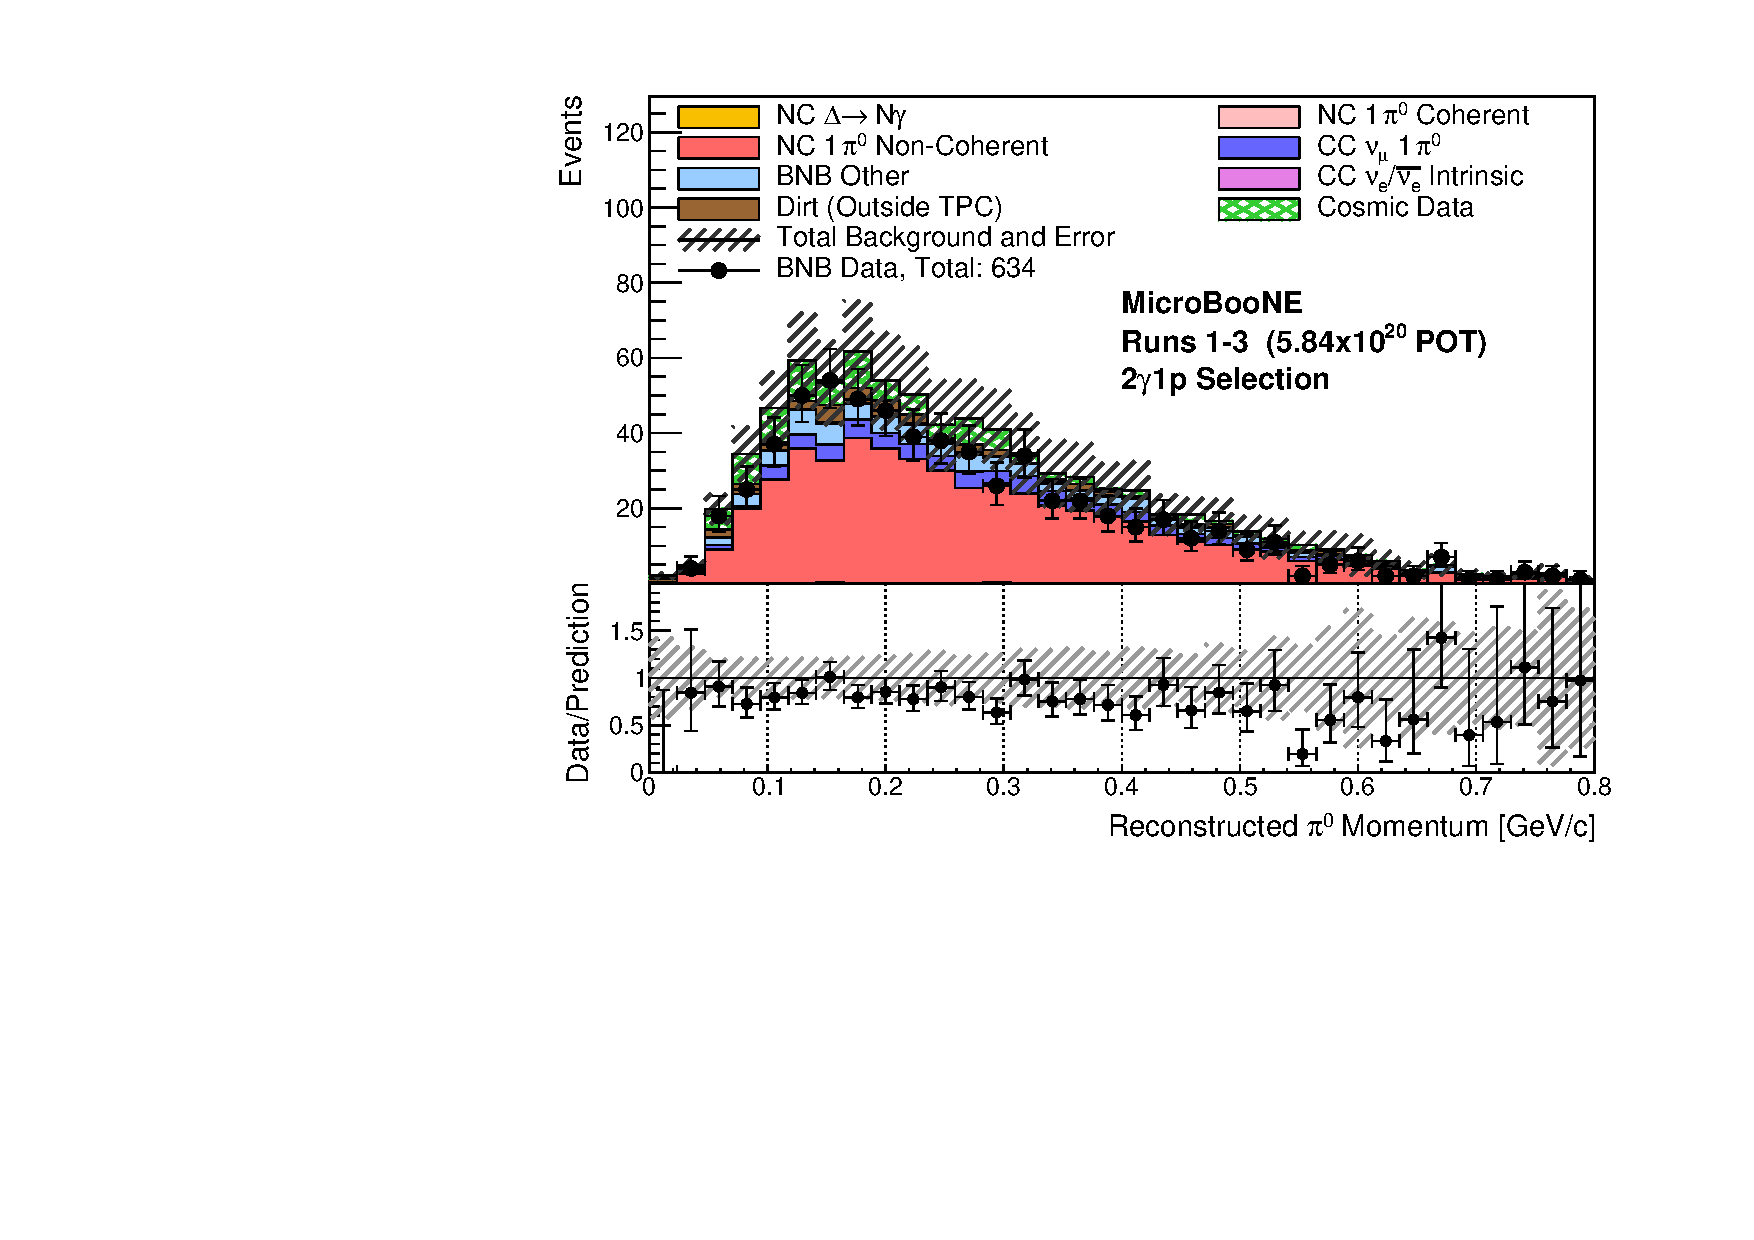
\includegraphics[width = \textwidth]{fig5a_pigLEE_combined_datamc_Data2g1pFiltered_Reconstructedpi0MomentumGeVc_stage_2WineCheese_v1.pdf}
        \vspace{-1cm}
        \caption{$2\gamma 1p$: Reconstructed $\pi^0$ momentum}
        %\caption{$2\gamma 1p$}
        \label{fig:ncpi0_mom_2g1p}
  \end{subfigure} 
    \begin{subfigure}{0.49\textwidth}
        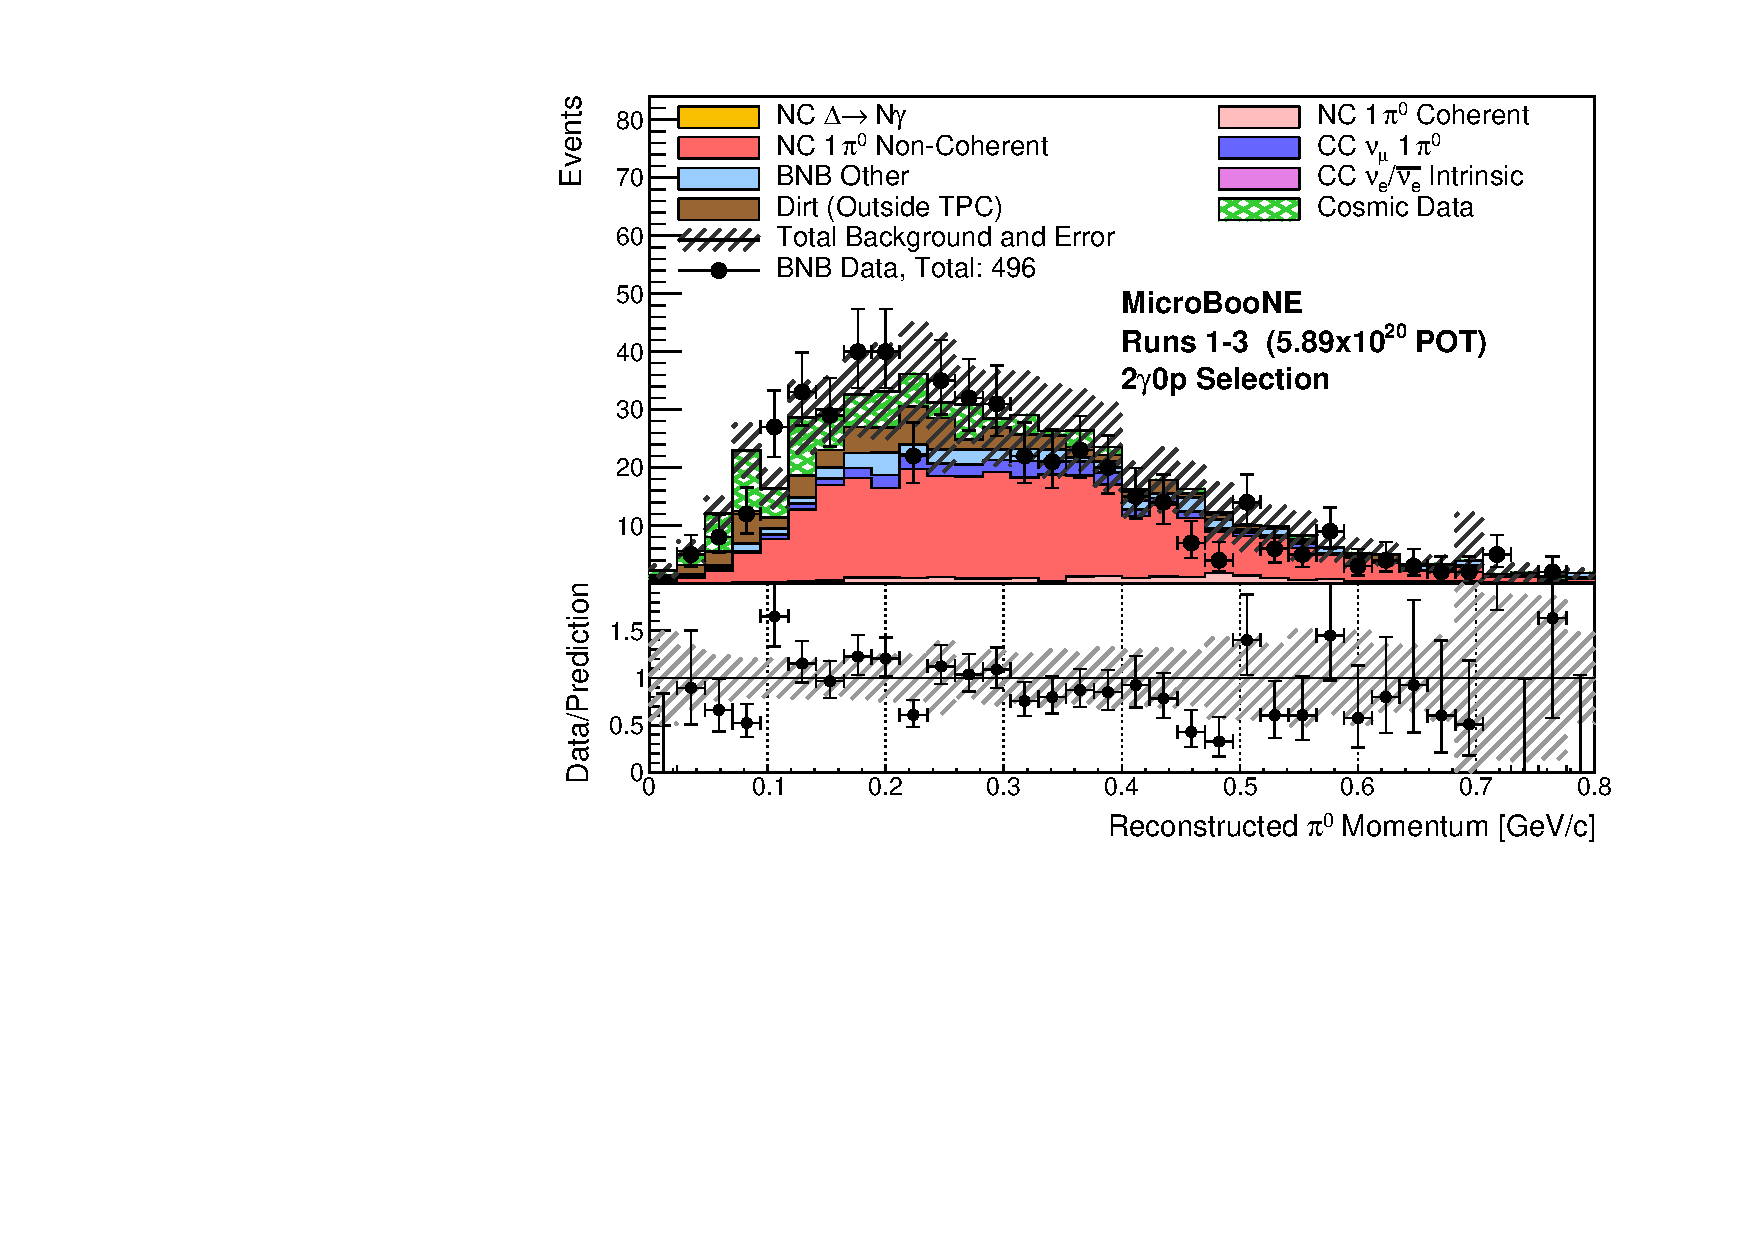
\includegraphics[width = \textwidth]{fig5b_pigLEE_2g0p_combined_datamc_Data2g0pFiltered_Reconstructedpi0MomentumGeVc_stage_2WineCheese_v1.pdf}
        \vspace{-1cm}
        \caption{$2\gamma 0p$: Reconstructed $\pi^0$ momentum}
        %\caption{$2\gamma 0p$}
        %\label{fig:ncpi0_mom_2g0p}
  \end{subfigure} 
    \begin{subfigure}{0.49\textwidth}
        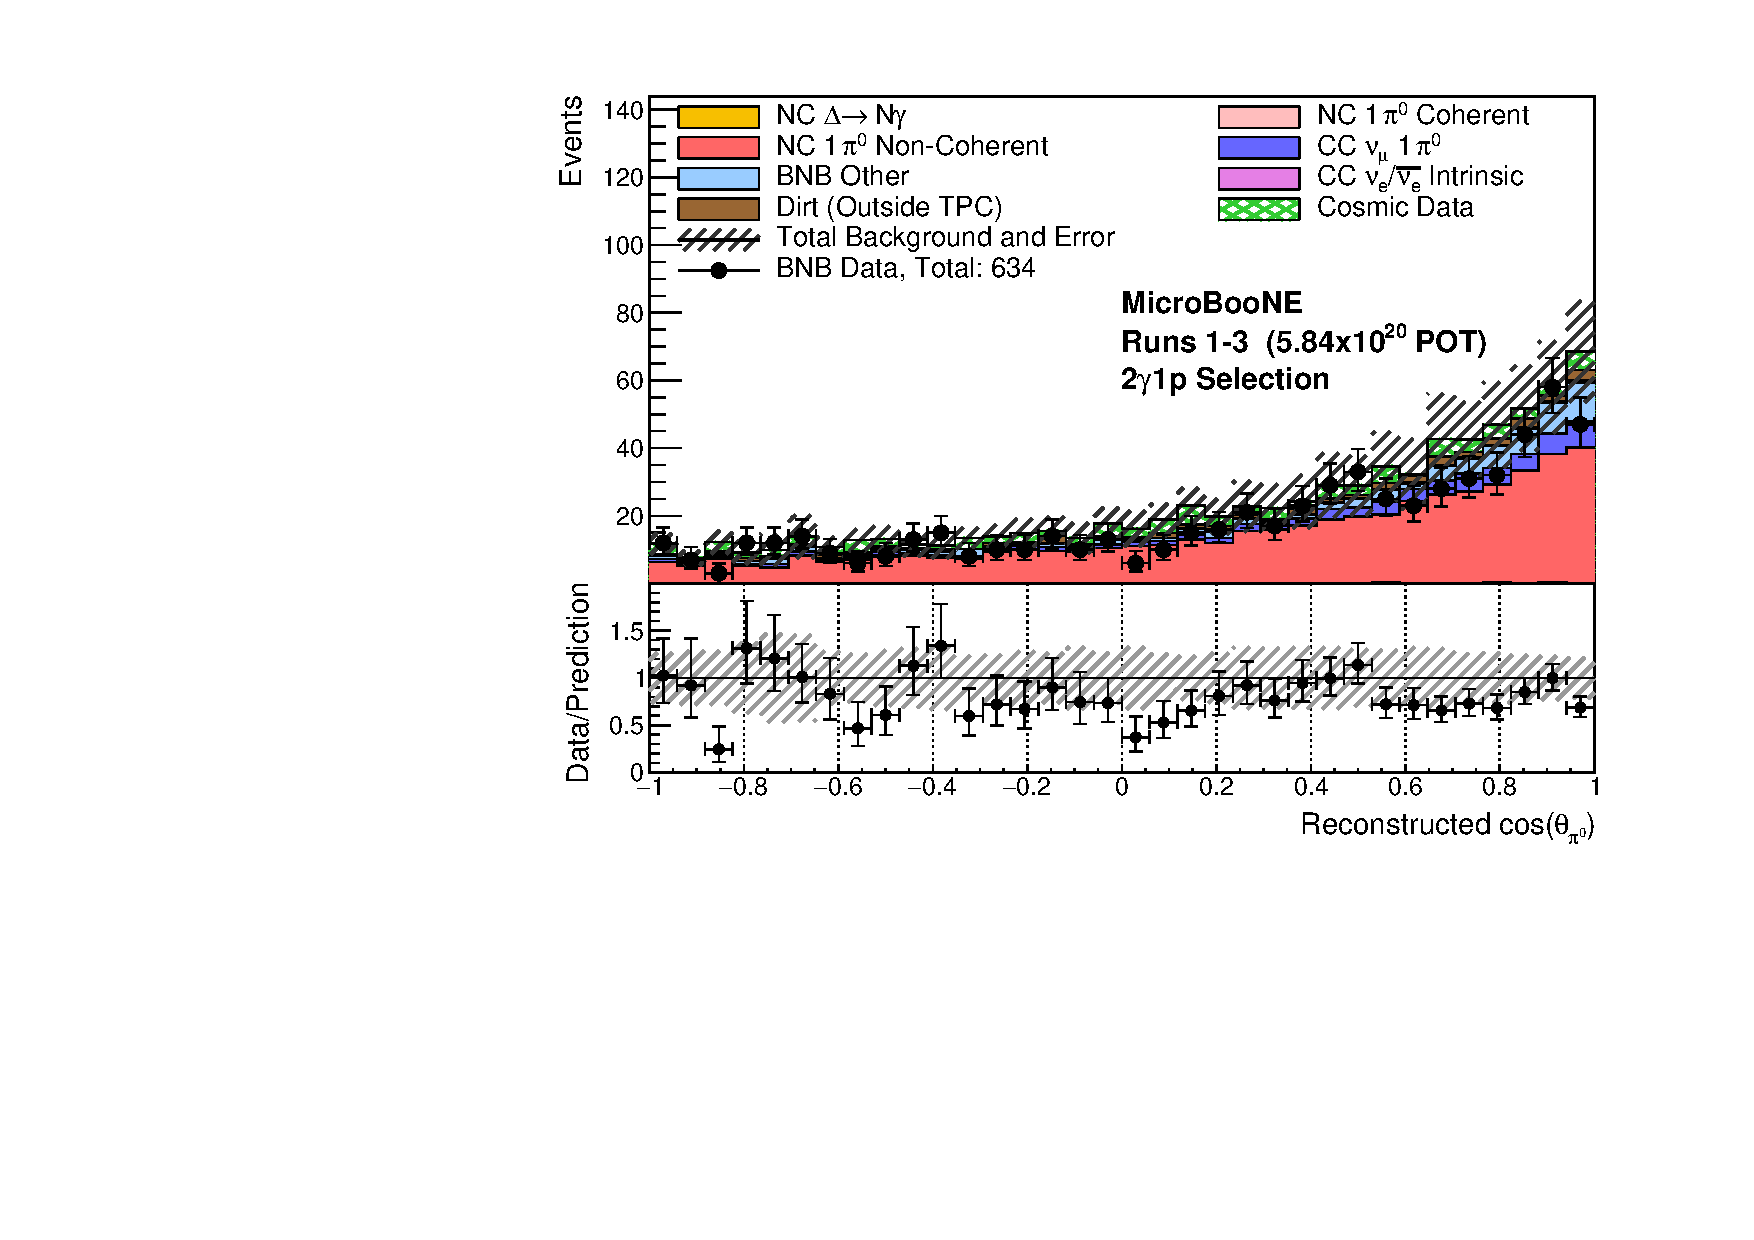
\includegraphics[width = \textwidth]{fig5c_pigLEE_combined_datamc_Data2g1pFiltered_Reconstructedcostheta_pi0_stage_2WineCheese_v1.pdf}
        \vspace{-1cm}
        \caption{$2\gamma 1p$: Reconstructed cosine of $\pi^0$ angle}
        %\caption{$2\gamma 1p$}
        %\label{fig:ncpi0_costheta_2g1p}
  \end{subfigure} 
  \begin{subfigure}{0.49\textwidth}
        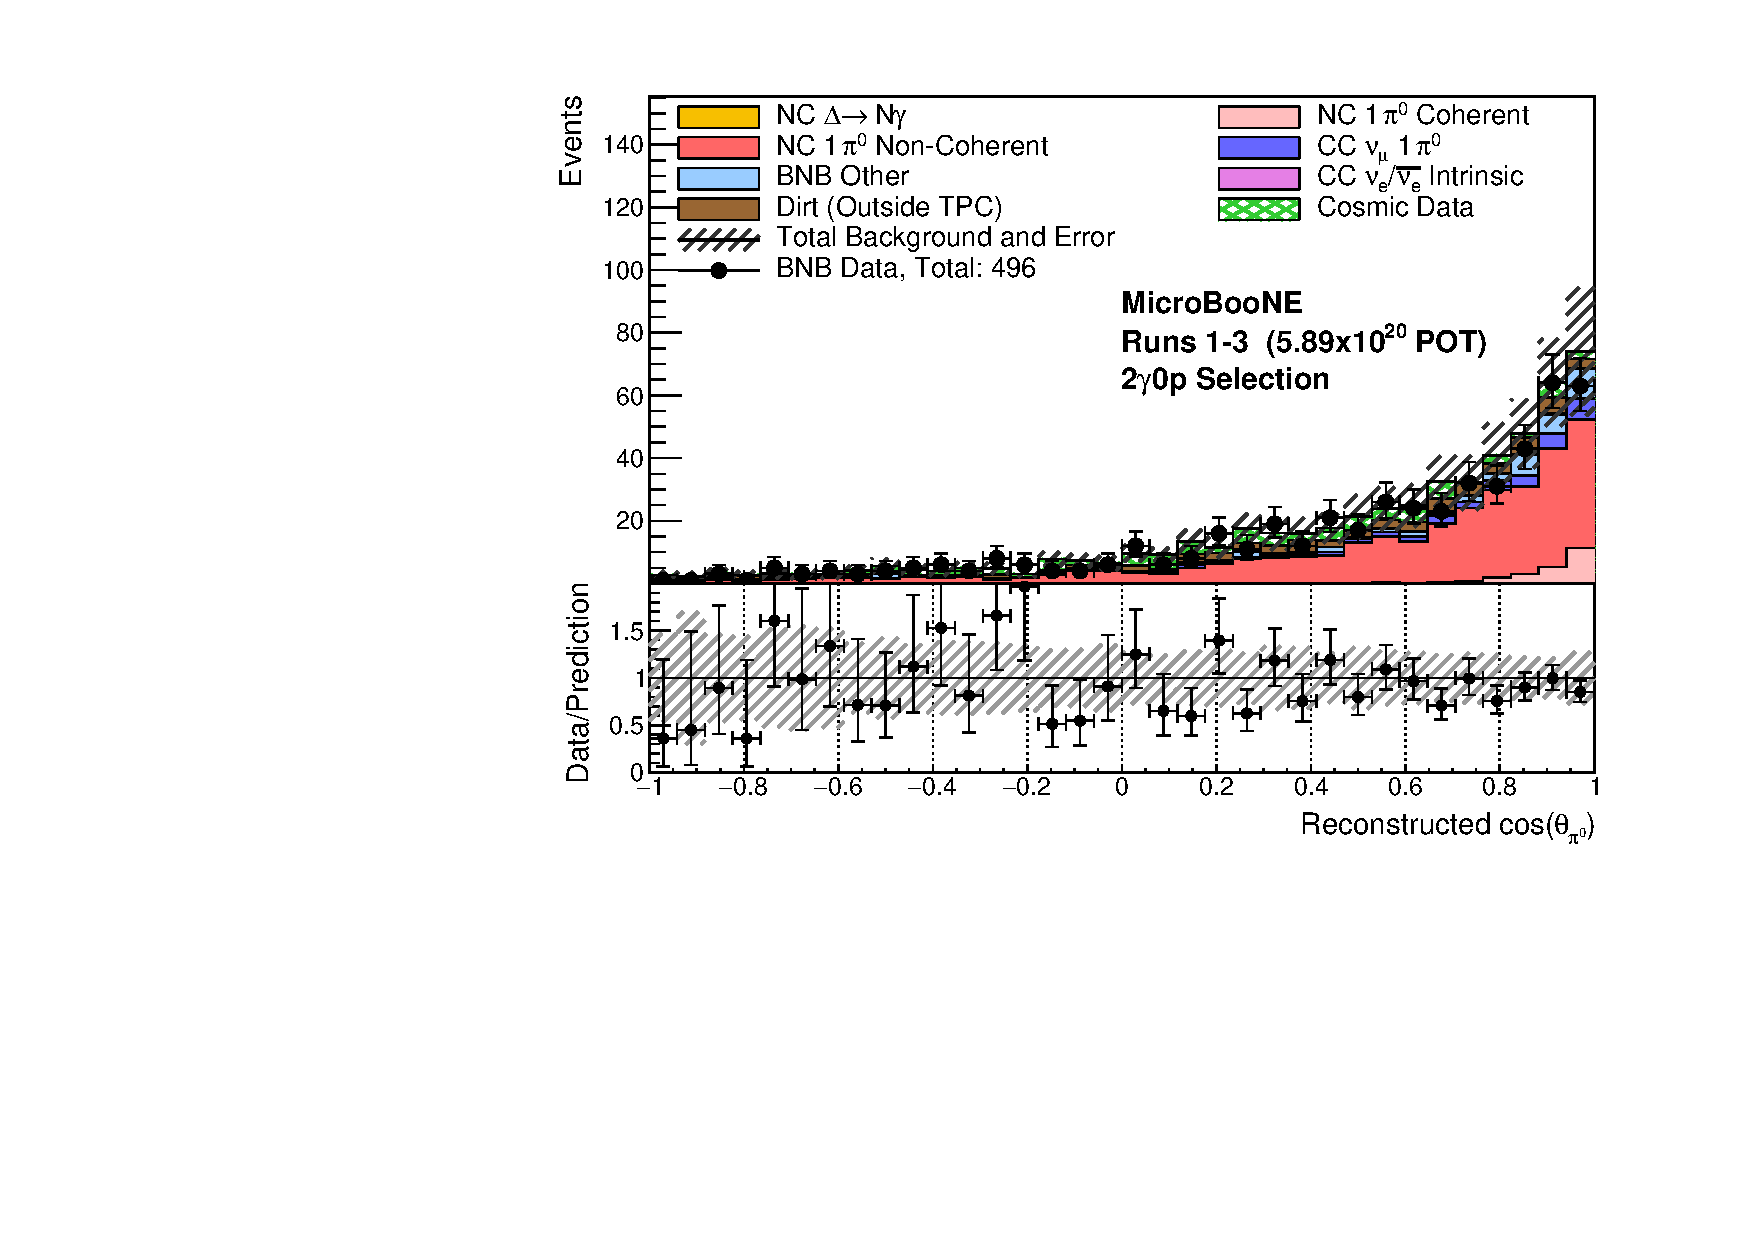
\includegraphics[width = \textwidth]{fig5d_pigLEE_2g0p_combined_datamc_Data2g0pFiltered_Reconstructedcostheta_pi0_stage_2WineCheese_v1.pdf}
        \vspace{-1cm}
        \caption{$2\gamma 0p$: Reconstructed cosine of $\pi^0$ angle}
        %\caption{$2\gamma 0p$}
        %\label{fig:ncpi0_costheta_2g0p}
  \end{subfigure}
  \caption{The reconstructed $\pi^0$ momentum ((a) and (b)) and reconstructed $\pi^0$ angle with respect to the neutrino beam ((c) and (d)) for both the $2\gamma1p$ ((a) and (c)) and $2\gamma0p$ ((b) and (d)) final selected data. The prediction shows agreement with the observed data within assigned uncertainties for the ranges shown, although a systematic deficit is observed in the total event rates as is discussed in Sec.~\ref{sec:deficit}.}
  \label{fig:ncpi0_costheta}
\end{figure*}

Two additional reconstructed distributions of interest are highlighted. First, the reconstructed cosine of the center-of-mass (CM) decay angle is shown in Fig.~\ref{fig:ncpi0_costhetacm}. This is defined as the angle between the lab-frame $\pi^0$ momentum direction and the decay axis of the two daughter photons in the CM frame, 
\begin{equation}
\cos\theta_\text{CM} =\frac{|E_{\gamma1} - E_{\gamma2}|}{|p_{\pi^0}|}. 
\label{eq:cos_theta}
\end{equation}

\noindent This quantity should be an isotropic flat distribution for true $\pi^0 \rightarrow \gamma\gamma$ signal events, and any deviation from this can highlight regions of inefficiency in reconstruction or selection. 
As can be seen in Fig.~\ref{fig:ncpi0_costhetacm}, for both $2\gamma1p$ and $2\gamma0p$ selections, the distributions taper off at high $\cos \theta_\text{CM}$ which corresponds to increasingly asymmetric $\pi^0$ decays. When reconstructing asymmetric $\pi^0$ decay events, it is more likely that the subleading photon shower is missed due to its low energy. Note, however, that the observed data show the same trend as the simulation within uncertainty.  

Figure~\ref{fig:ncpi0_conv} additionally highlights the reconstructed photon conversion distance for all showers in the final $2\gamma1p$ selection.  Well-reconstructed showers with conversion distances as far as 100~cm from the candidate neutrino interaction are observed. This helps validate the assumption that the reconstructed showers are indeed likely to be true photons as $\mathcal{O}$(100)~MeV photons are expected to have a mean free path in argon of $\approx 20$~cm.  Note that, as the $2\gamma0p$ selection does not have any visible hadronic activity for tagging the interaction point, the corresponding conversion distance is significantly harder to estimate.

\begin{figure}[h]
    \centering 
    \begin{subfigure}{0.49\textwidth}
        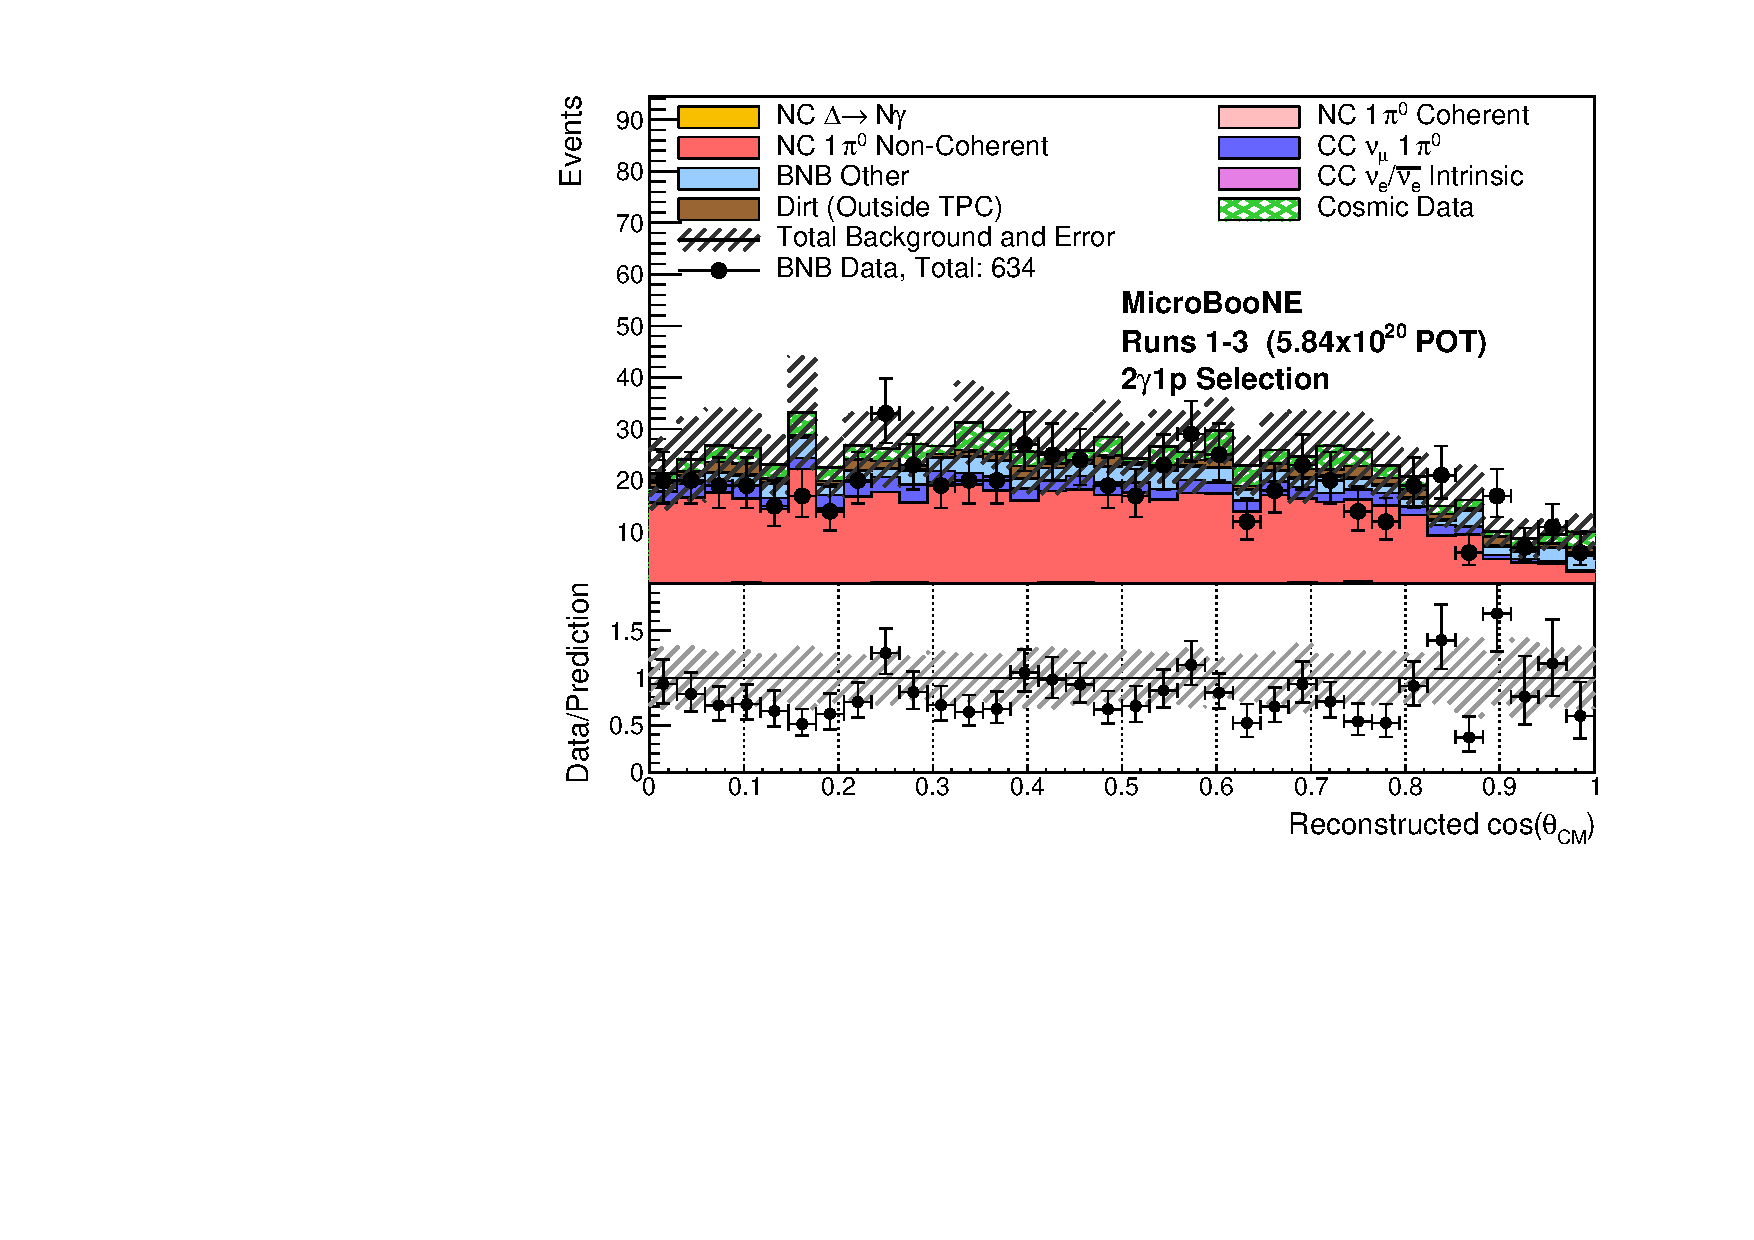
\includegraphics[width = \textwidth]{fig6a_pigLEE_combined_datamc_Data2g1pFiltered_Reconstructedcostheta_CM_stage_2WineCheese_v1.pdf}
        \vspace{-1cm}
       \caption{$2\gamma 1p$}
      %  \label{fig:ncpi0_invar_2g1p}
  \end{subfigure} 
  \begin{subfigure}{0.49\textwidth}
        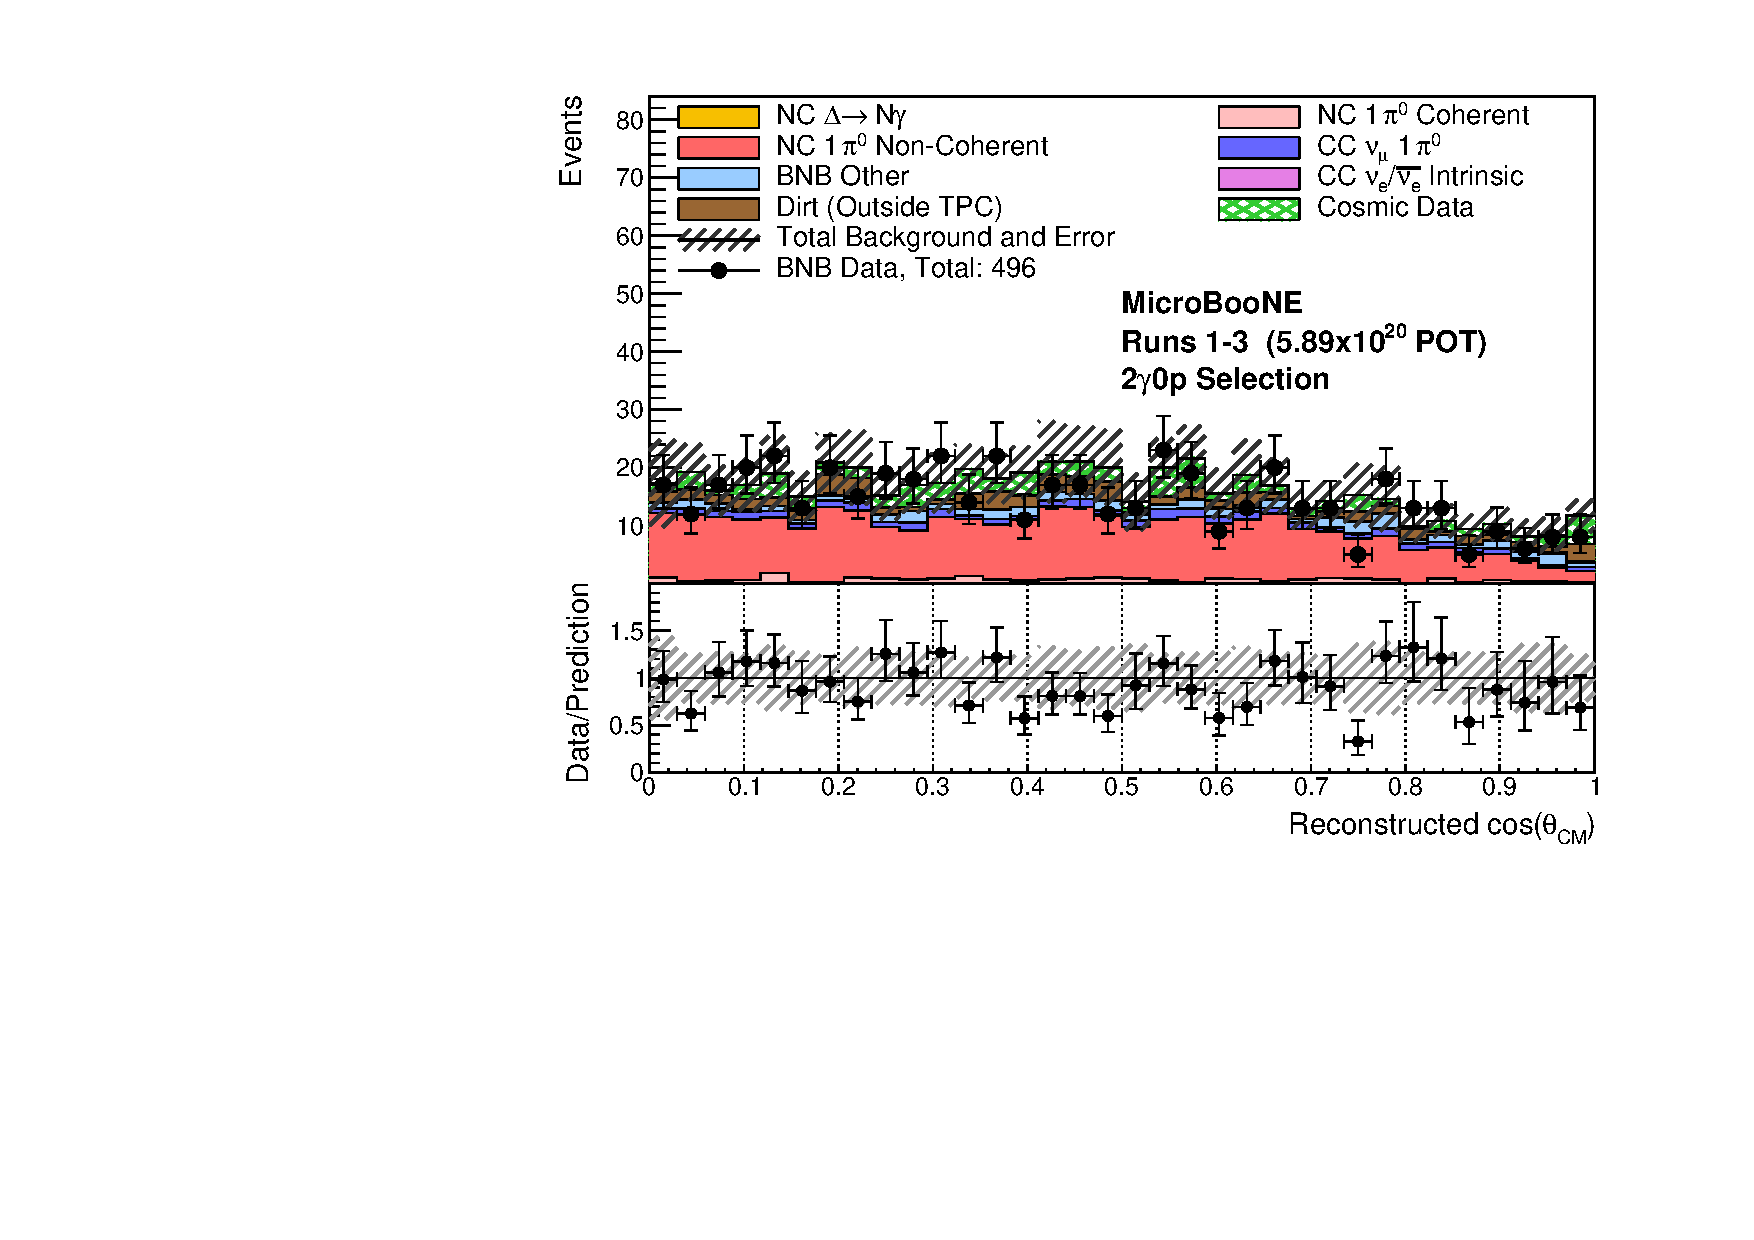
\includegraphics[width = \textwidth]{fig6b_pigLEE_2g0p_combined_datamc_Data2g0pFiltered_Reconstructedcostheta_CM_stage_2WineCheese_v1.pdf}
        \vspace{-1cm}
        \caption{$2\gamma 0p$}
    %    \label{fig:ncpi0_invar_2g0p}
  \end{subfigure}
  \caption{The reconstructed cosine of the center-of-mass angle for the (a) $2\gamma1p$ and (b) $2\gamma0p$ final selected data.}
  \label{fig:ncpi0_costhetacm}
\end{figure}

\begin{figure}[h!]
    \centering 
    \begin{subfigure}{0.49\textwidth}
        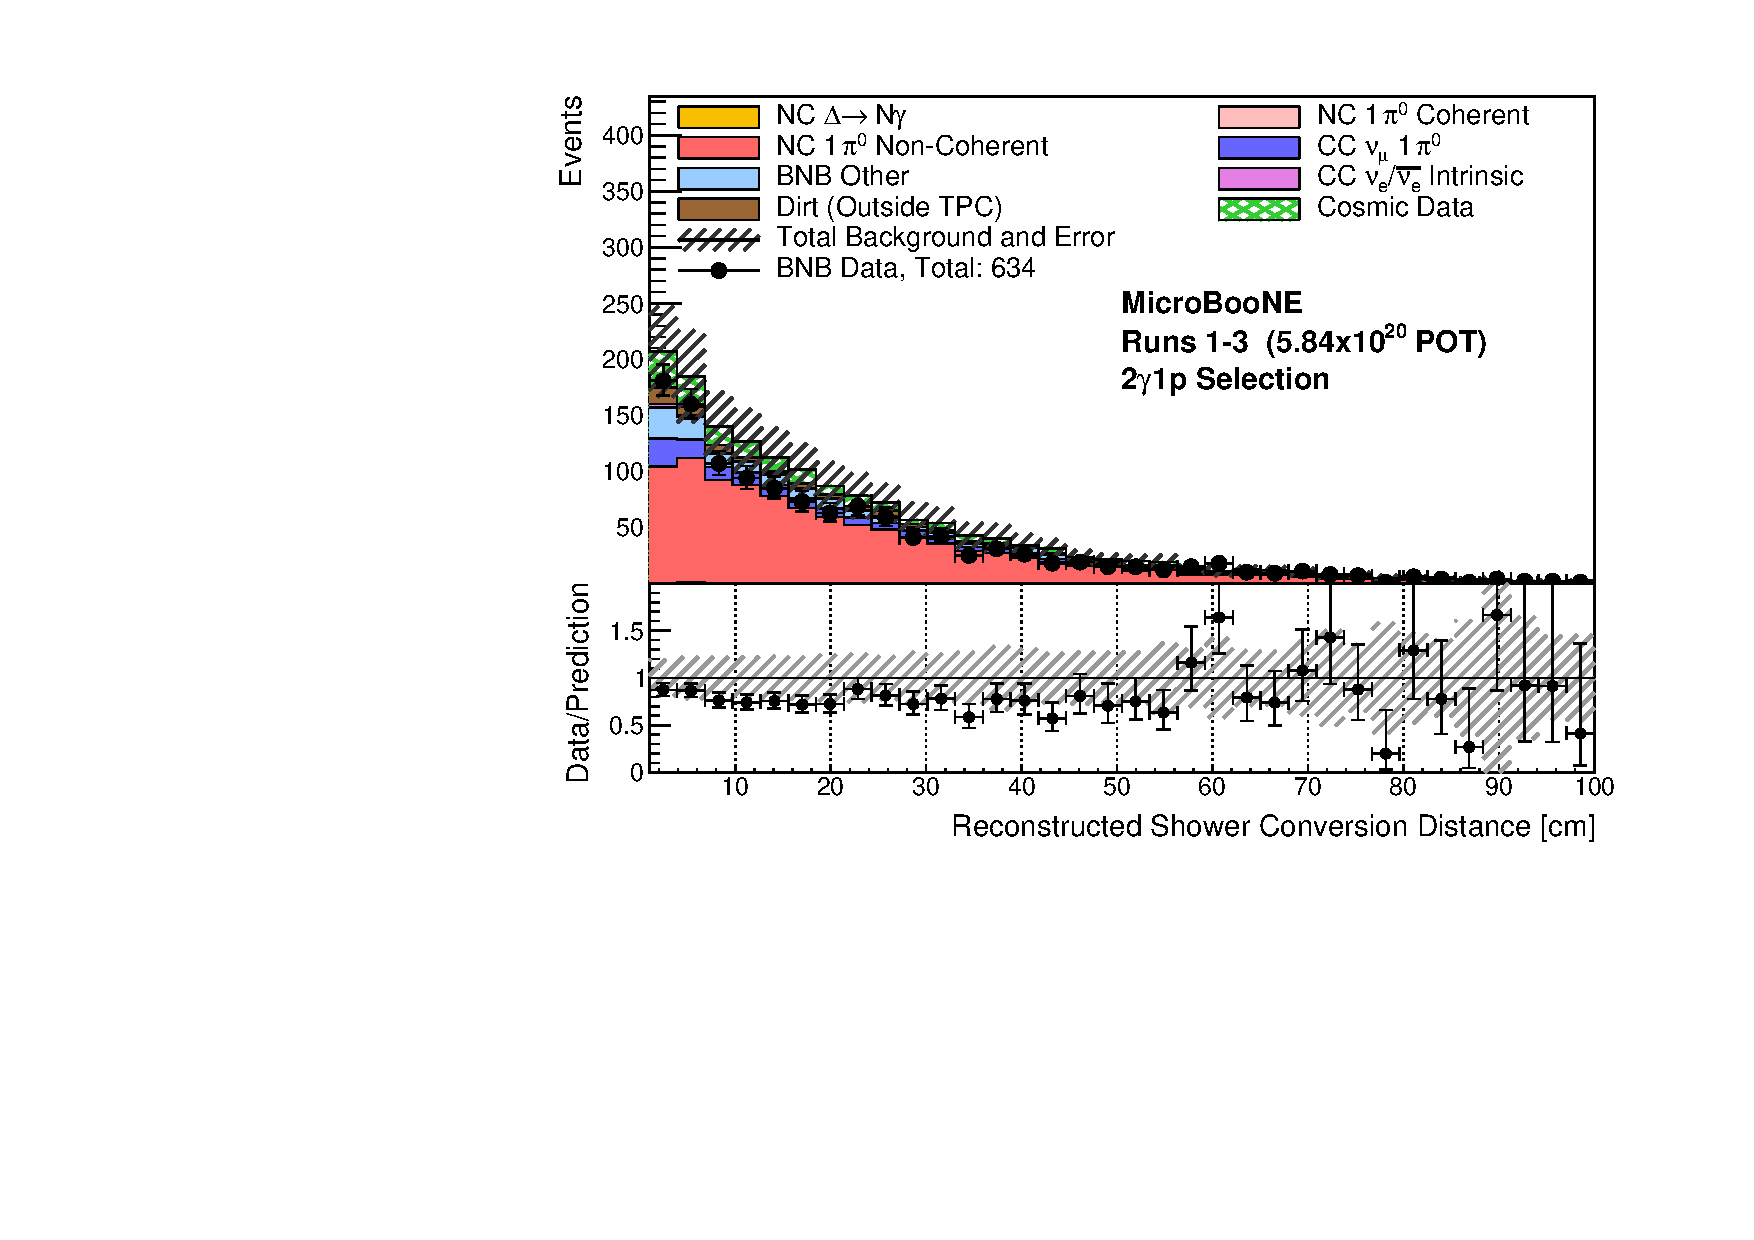
\includegraphics[width = \textwidth]{fig7_pigLEE_combined_datamc_Data2g1pFiltered_ReconstructedShowerConversionDistancecm_stage_2WineCheese_v1.pdf}
  \end{subfigure} 
  \caption{The reconstructed conversion distance of both photons in the $2\gamma1p$ final selection.  There are well-reconstructed showers with conversion distances as far as 100~cm from the candidate neutrino interaction.}
  \label{fig:ncpi0_conv}
\end{figure}

Finally, Fig.~\ref{fig:ncpi0_evds} shows two example event displays of selected events in data for both the $2\gamma 1p$ and $2\gamma 0p$ topologies. Each event shows two well-reconstructed showers pointing back to a common interaction point with properties consistent with those being photons from a $\pi^0$ decay.

\begin{figure}
    \centering
    \begin{subfigure}{0.44\textwidth}
        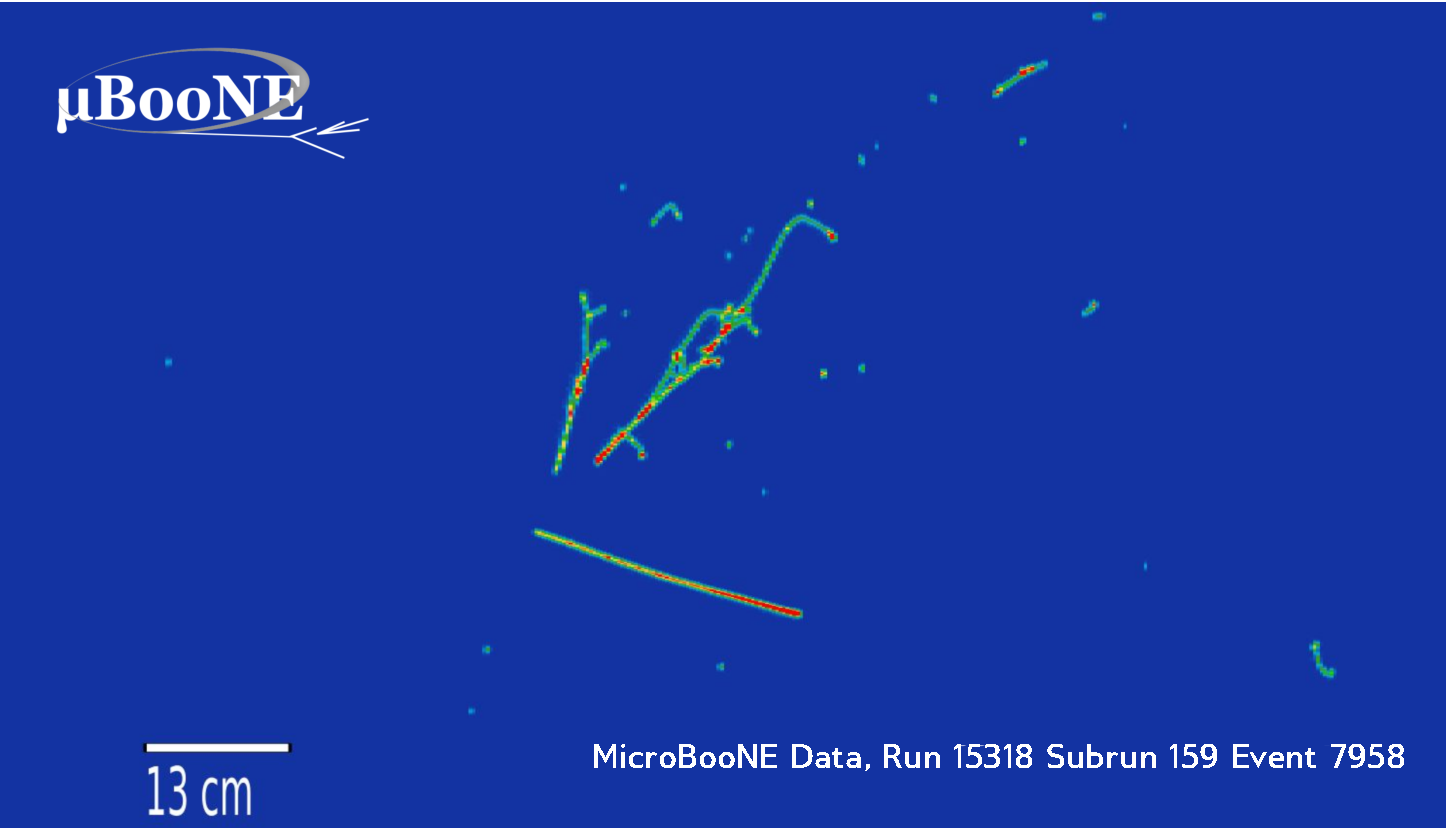
\includegraphics[width=\textwidth]{fig8a_2g1p_evd_15318_159_7958_fixed.pdf}
        \caption{$2\gamma 1p$}
        \label{fig:2g1p_evd}
    \end{subfigure}
    \begin{subfigure}{0.44\textwidth}
        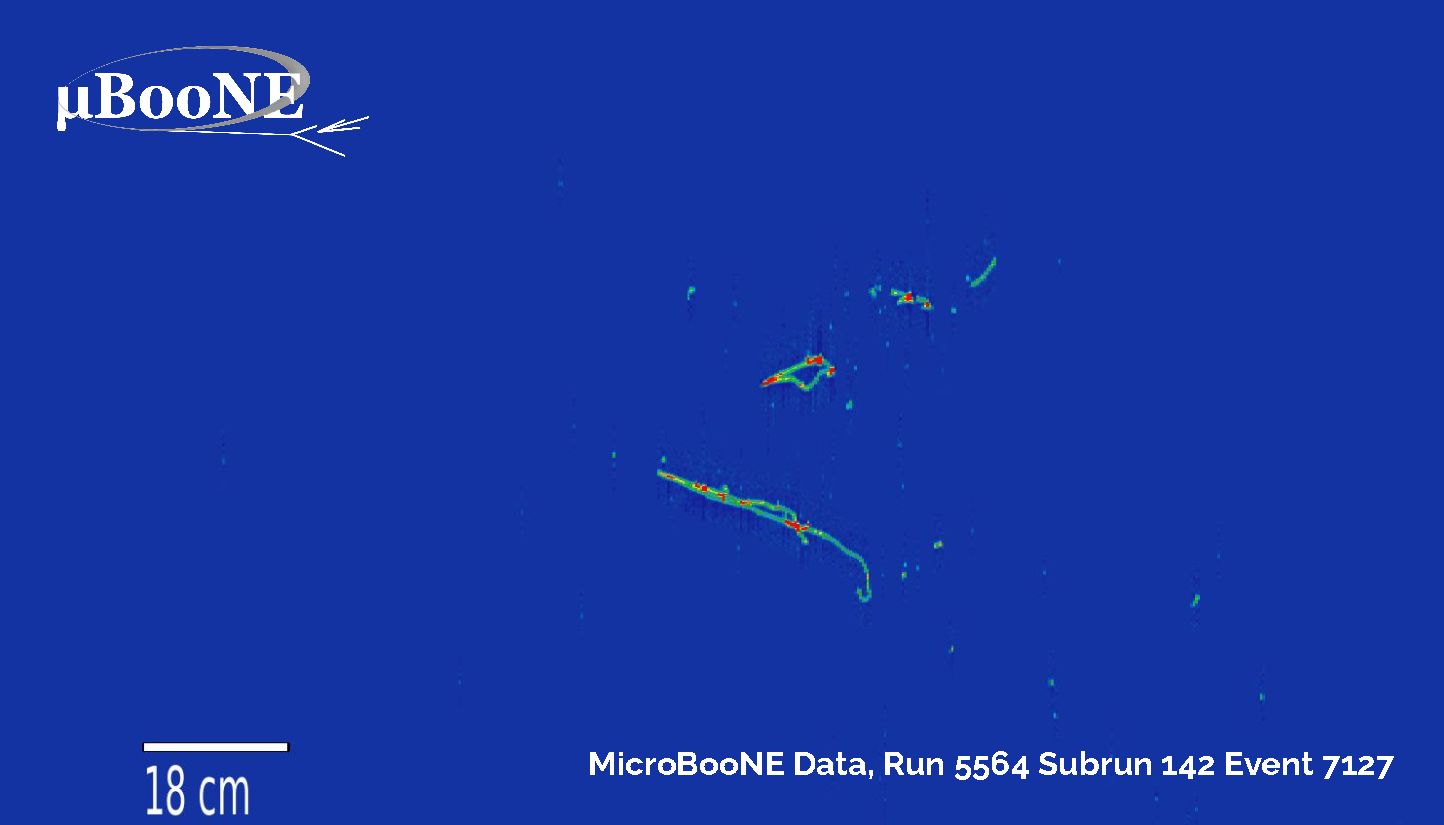
\includegraphics[width=\textwidth]{fig8b_2g0p_evd_5564_142_7127.pdf}
        \caption{$2\gamma 0p$}
        \label{fig:2g0p_evd}
    \end{subfigure}
    \caption{Event displays of candidate NC $1\pi^0$ events found in the MicroBooNE data using (a) the $2\gamma 1p$ selection and (b) the $2\gamma 0p$ selection, on the MicroBooNE TPC collection plane. The horizontal axis here corresponds to the increasing wires, with an associated distance in cm. The vertical axis represents the TPC drift time. The aspect ratio of this plot is set such that the length scale shown for the horizontal axis is the same for the vertical axis.}
    \label{fig:ncpi0_evds}
\end{figure}

\subsection{Background Discussion and Validation}
\label{sec:backgrounds}
In order to validate the background modelling in this analysis we developed a background rich sideband selection by inverting the BDT score cuts shown in Fig.~\ref{fig:bdt_responses}. This gives us a high statistics sample of ``CC$1\pi^0$'' and ``BNB Other'' background categories with which to compare to data. In addition to inverting the BDT score an additional cosmic rejection cut, where we require the Pandora neutrino score to be $>0.5$, is applied to provide a higher purity of the backgrounds we wish to study. These distributions are shown in Fig.~\ref{fig:bkg_study_1p} and ~\ref{fig:bkg_study_0p} for $2\gamma1p$ and $2\gamma0p$ respectively. This is particularly useful for $2\gamma1p$ inverted selection as the resulting spectrum is rich in CC$1\pi^0$ for higher reconstructed $\pi^0$ momenta, and richer in ``BNB Other'' at low momenta. For the $2\gamma0p$ background rich sample there is still a significant amount of rejected NC $\pi^0$ signal events, but the enhanced backgrounds still provide additional validation. The data is observed to be in good agreement with the prediction, within assigned uncertainties, with a $\chi^2/\text{ndof}$ of $24.61/20$ and $17.49/22$ for $2\gamma1p$ and $2\gamma0p$ respectively. This gives us confidence that the backgrounds and uncertainties are sufficiently modelled for a cross-section extraction to proceed.

We can also break down the ``BNB Other'' category further in order to improve our understanding of this important background. We find that approximately $75\%$ of ``BNB Other'' events contain true photons reconstructed, and in case of $2\gamma1p$ 84\% have true protons reconstructed. This indicates that despite being a background category the BDT's are indeed selecting events with a very high purity of true photons and protons, as is the target of the selection. The approximate breakdown of ``BNB Other'' after applying the BDT cuts is found to be

\begin{itemize}
    \item $\approx 25\%$ are events in which multiple $\pi^0$ are exiting the nucleus but only 1 $\pi^0$ is reconstructed correctly,
    \item $\approx 25\%$ are events in which no $\pi^0$ exits the nucleus but due to baryon or charged pion re-scattering in the argon, a $\pi^0$ is subsequently created and reconstructed,  
    \item $\approx 25\%$ are events in which there is no $\pi^0$ and a NC proton is reconstructed as the track with cosmic contamination resulting in a $2\gamma$ event mimicking a $\pi^0$,
    \item $\approx 20\%$ are events containing a NC $\eta \rightarrow \gamma \gamma$ decay event. These are generally rejected due to them having higher energies, but a small number are selected as they are topologically identical to the $\pi^0\rightarrow \gamma\gamma$ decay signal, 
    \item $\approx 5\%$ Miscellaneous other reconstruction failures, representing less than 1\% of total background events.  
\end{itemize}

In the case of CC$1\pi^0$ we see a similar situation, with 97.3\% (98.1\%) of $2\gamma1p$  ($2\gamma0p$) background events having at least 1 shower matched to a true $\pi^0$ and with 78\% of tracks in the $2\gamma1p$ sample being correctly matched to a proton. As such, the vast majority of these events have the correct target particle content, but rather the muon itself is missed. This primarily occurs when the muon is incorrectly clustered into a photon electro-magnetic shower due to close proximity, or when the muon is correctly reconstructed but is mis-identified as a cosmic muon, with the associated $\pi^0$ then being reconstructed as an isolated neutrino event.

\begin{figure}[h]
    \centering 
    \begin{subfigure}{0.49\textwidth}
        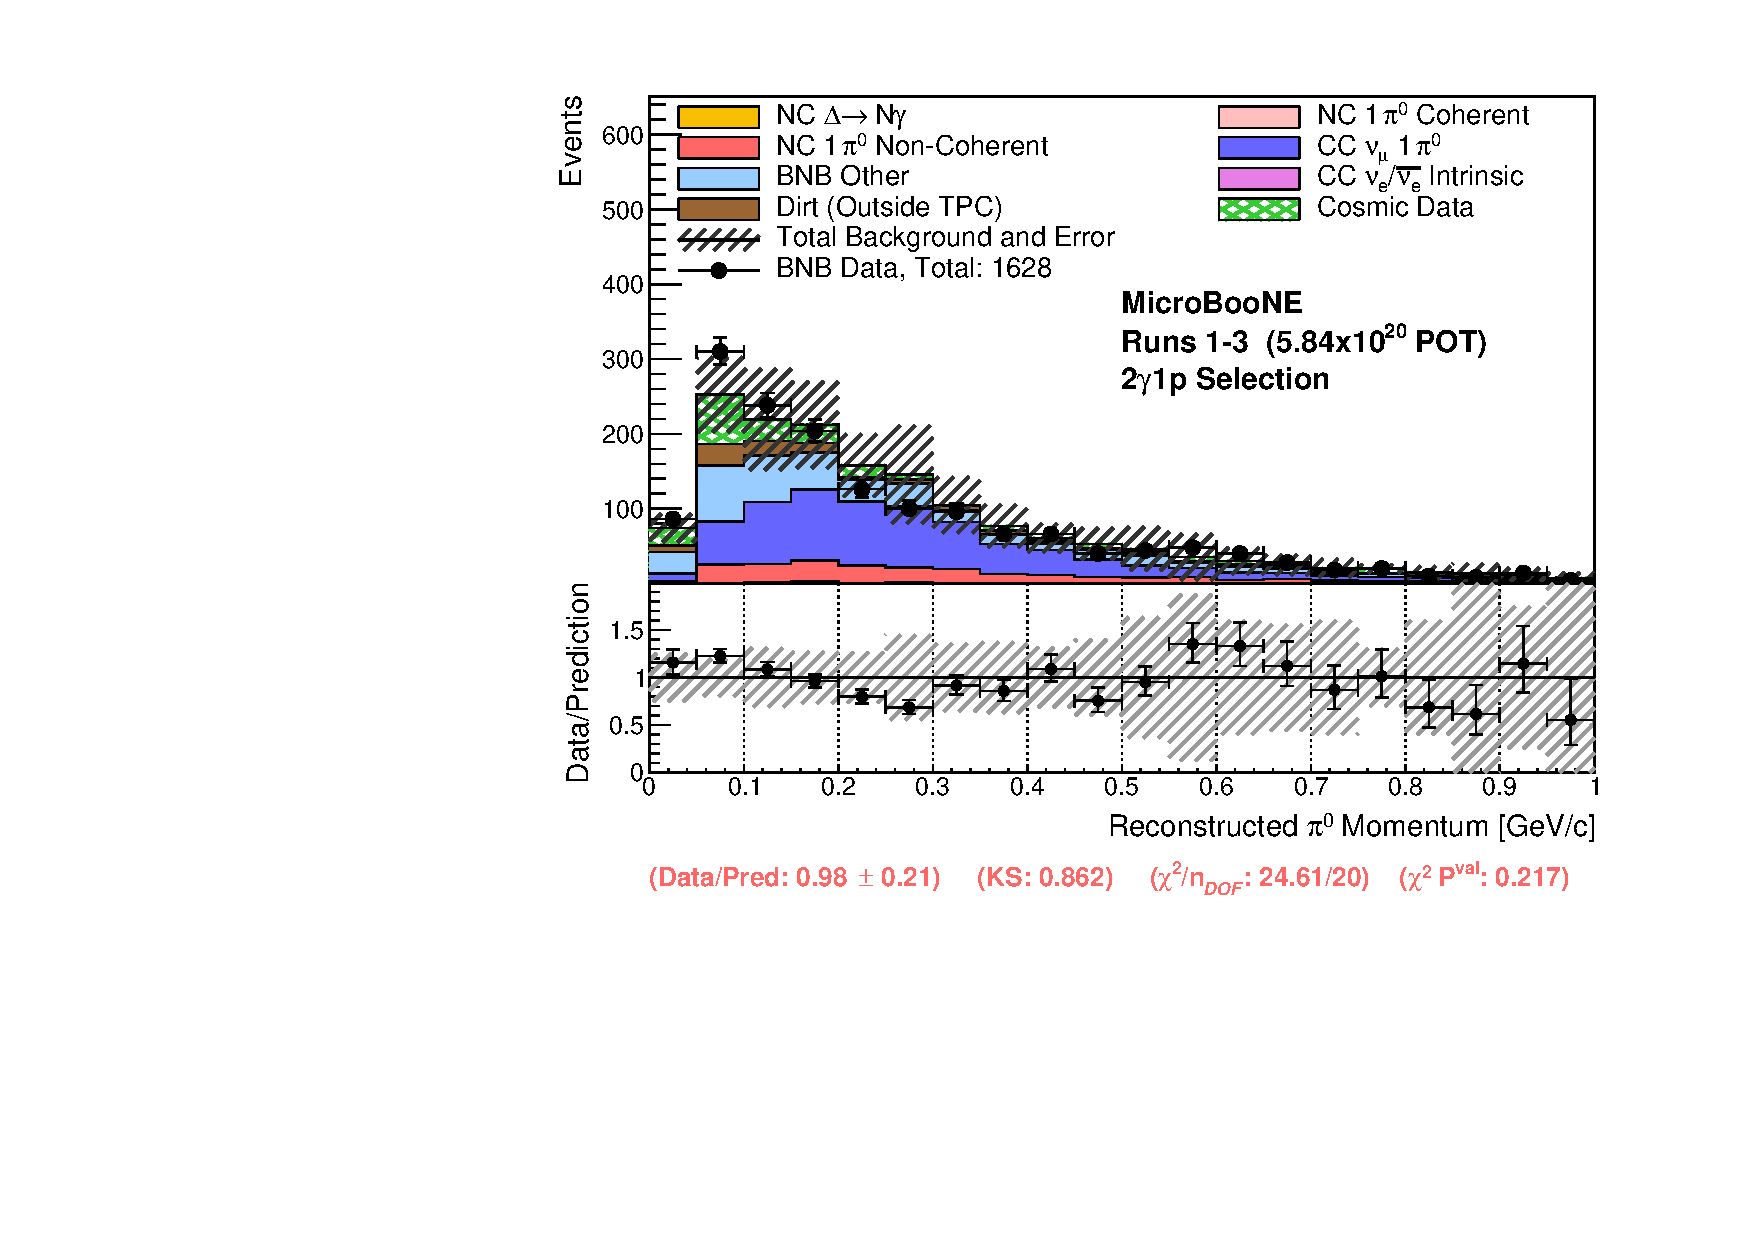
\includegraphics[trim={0 1.5cm 0 0},clip, width = \textwidth]{fig9a_pigLEE_combined_datamc_Data2g1pFiltered_Reconstructedpi0MomentumGeVc_stage_1WineCheese_v1_REF_BGROUND_FIN.pdf}
        %\vspace{-1cm}
       \caption{$2\gamma 1p$ background validation sample}
        \label{fig:bkg_study_1p}
  \end{subfigure} 
  \begin{subfigure}{0.49\textwidth}
      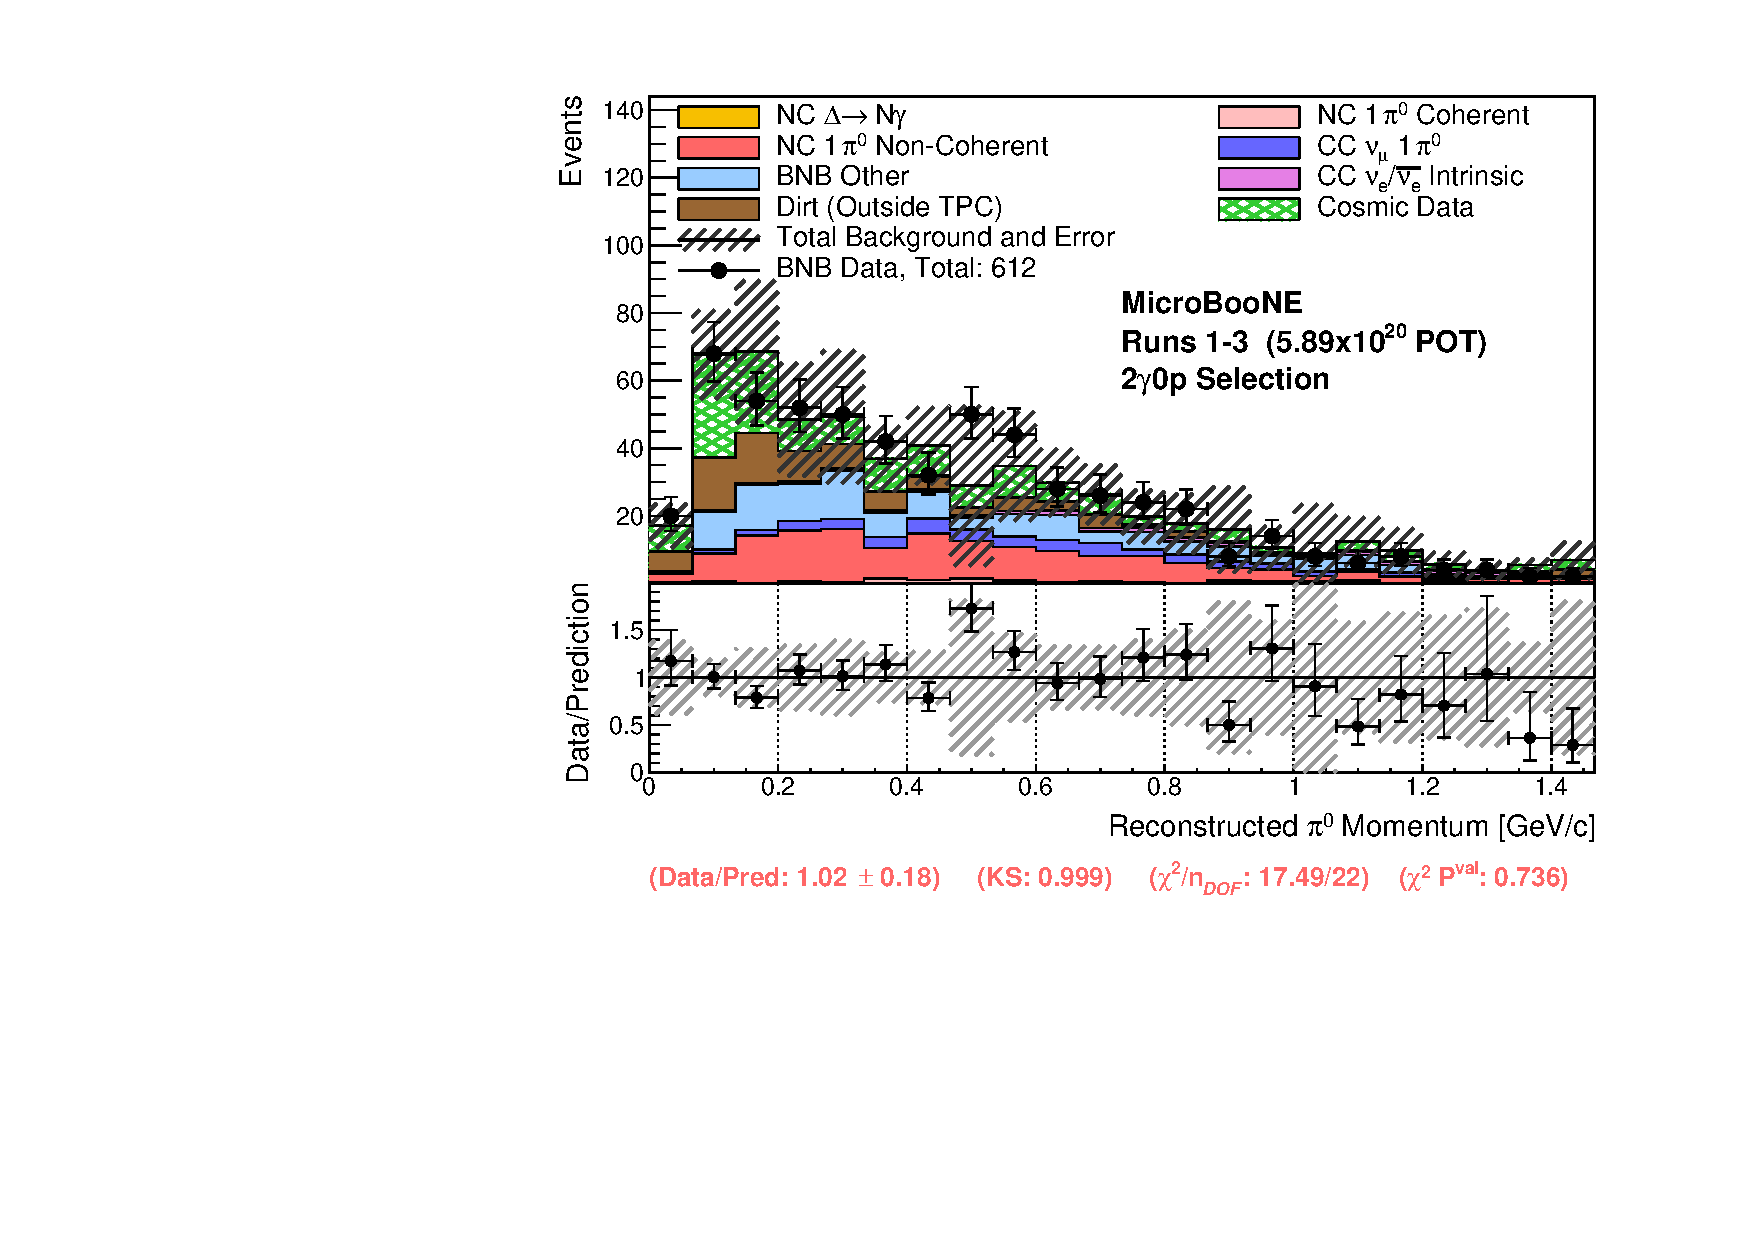
\includegraphics[trim={0 1.5cm 0 0},clip, width = \textwidth]{fig9b_pigLEE_2g0p_combined_datamc_Data2g0pFiltered_Reconstructedpi0MomentumGeVc_stage_1WineCheese_v1_REF_BGROUND_FIN.pdf}
        %\vspace{-1cm}
        \caption{$2\gamma 0p$ background validation sample}
        \label{fig:bkg_study_0p}
  \end{subfigure}
  \caption{Background rich sidebands for validation created by inverting the BDT selection cuts, for (a) $2\gamma1p$ and (b) $2\gamma0p$ samples. We observe good agreement between the data and prediction, within the assigned uncertainties giving us confidence in the background modelling.}
  \label{fig:bkg_study}
\end{figure}
